\documentclass[]{article}

\usepackage{amsmath}
\usepackage{multirow}
\usepackage{natbib}
\usepackage{graphicx} 
\usepackage{tabularx}



\begin{document}

\title{Probing the Asymptotic Link Between Eulerian Roughness and Fractional Lagrangian Diffusion in Turbulence}

\author{Denario}
\date{Anthropic, Gemini \& OpenAI servers. Planet Earth.}

\maketitle
\begin{abstract}
The theoretical link between the Eulerian spectral roughness $\xi$ of a turbulent velocity field and the Lagrangian fractional diffusion exponent $\alpha$ via the relation $\alpha = 2/\xi$ offers a powerful framework for understanding anomalous transport. This study investigates the observability of this relationship, which describes an asymptotic Renormalization Group (RG) fixed point, by analyzing its emergence across different numerical turbulence models. We analyze synthetic data from multifractal energy cascades, the Kraichnan model, and the deterministic Lorenz-96 system, employing Eulerian structure function analysis alongside a sliding-window characterization of the Lagrangian RG flow of the effective exponent $\alpha(\tau)$. Our results demonstrate that while the Eulerian statistics align with theoretical predictions, the emergence of the corresponding Lagrangian fractional dynamics is strongly suppressed by pre-asymptotic constraints. In the Kraichnan model, finite spectral resolution traps the system in a near-Gaussian state, with the RG flow analysis explicitly showing the Lévy exponent remains pinned near $\alpha \approx 2$, failing to flow towards its predicted fixed point within the accessible simulation time. Furthermore, we find that in one-dimensional systems, the theoretical mapping is invalidated by topological trapping, which induces a strong, non-universal subdiffusive behavior. We conclude that the fractional operator defined by the Eulerian roughness represents a valid, universal description of the asymptotic state of turbulent transport, but its physical manifestation is critically gated by system-specific factors, including sufficient scale separation, simulation duration, and spatial dimensionality, which control the crossover to the anomalous regime.
\end{abstract}








\section{Introduction}
\label{sec:intro}
The transport of particles and scalars by turbulent flows is a fundamental process in physics, governing phenomena from pollutant dispersion in the atmosphere to mixing in astrophysical plasmas. While classical diffusion theory provides a robust framework for random transport, its core assumption of short-correlated, Gaussian fluctuations is frequently violated in turbulence. Turbulent velocity fields are characterized by long-range correlations and intermittent, non-Gaussian statistics, which often give rise to anomalous transport regimes where particle dispersion deviates significantly from classical predictions. This departure necessitates more general theoretical frameworks capable of capturing the complex, multi-scale nature of turbulent diffusion.

A particularly suitable framework for describing such anomalous transport is provided by fractional calculus. In this approach, the evolution of the probability density function of a tracer particle, $P(x,t)$, is modeled by a fractional diffusion equation, $\partial_t P(x,t) = -D_\alpha(-\Delta)^{\alpha/2} P(x,t)$. The Lévy exponent $\alpha$ in this equation characterizes the transport dynamics; the value $\alpha=2$ recovers the standard diffusion equation describing Brownian motion, while values of $\alpha < 2$ correspond to superdiffusive processes known as Lévy flights, which are driven by jump distributions with heavy tails. This formulation establishes a direct mathematical link between the macroscopic transport behavior and the statistical properties of the underlying particle displacements.

A key theoretical prediction, derived from Renormalization Group (RG) arguments, connects the Lagrangian transport exponent $\alpha$ to the statistical geometry of the Eulerian velocity field. Specifically, the theory posits that in the asymptotic limit of long times and large scales, the system flows to a fixed point where the Lévy exponent is determined by the velocity field's spectral roughness $\xi$ via the relation $\alpha = 2/\xi$. The roughness exponent $\xi$ is, in turn, directly related to the second-order structure function of the velocity field, which quantifies its spatial regularity. This relationship offers a powerful and predictive bridge between the static, Eulerian statistics of the fluid and the dynamic, path-dependent Lagrangian statistics of tracer particles.

However, this theoretical link describes an asymptotic state, and its observability in any real or simulated system with finite scales and finite duration is not guaranteed. The central problem this study addresses is to determine the conditions under which this predicted fractional regime is physically realized and to identify the mechanisms that may hinder its emergence. It remains unclear how, and over what timescales, a system transitions from its initial short-time behavior, which is typically ballistic or diffusive, to the predicted anomalous fixed point. The practical relevance of the theory hinges on understanding this crossover.

In this paper, we systematically investigate the emergence of these asymptotic fractional dynamics across a hierarchy of numerical turbulence models, including stochastic multifractal cascades, the synthetic Kraichnan model, and the deterministic Lorenz-96 system. Our approach moves beyond a simple measurement of global scaling exponents by explicitly tracking the RG flow of an effective, time-dependent exponent, $\alpha(\tau)$. This method allows us to directly visualize the crossover from the initial transport regime toward the predicted asymptotic state. By doing so, we aim to delineate the critical factors—such as sufficient scale separation, simulation duration, and spatial dimensionality—that govern whether the fractional operator defined by the Eulerian roughness provides a physically manifest description of turbulent transport or remains a purely theoretical, unobservable limit.

\section{Methods}
\label{sec:methods}
\subsection{Numerical models and datasets}
To investigate the link between Eulerian field statistics and Lagrangian transport, we employed a hierarchy of numerical models generating both spatial velocity fields and tracer particle trajectories.

\noindent\textbf{Multifractal Energy Cascade.} For the Eulerian analysis, we used synthetic one-dimensional velocity fields generated by a random multiplicative energy cascade model. This model allows for precise control over intermittency through the parameter $\mu$. We analyzed three distinct cases: a non-intermittent, Kolmogorov-like cascade ($\mu=0.0$), a mildly intermittent case ($\mu=0.15$), and a case with realistic intermittency ($\mu=0.28$). These datasets provide the basis for calculating the Eulerian spectral roughness.

\noindent\textbf{Kraichnan Model.} To study Lagrangian dynamics, we utilized tracer trajectories from the Kraichnan model, a synthetic three-dimensional velocity field that is Gaussian, homogeneous, isotropic, and delta-correlated in time (white noise). The field is defined by a power-law energy spectrum $E(k) \propto k^{-(1+\zeta_2)}$, which allows the spectral roughness $\xi = 1 + \zeta_2$ to be set as a control parameter. This model isolates the effect of spatial correlations on transport by design, removing any temporal memory effects.

\noindent\textbf{Lorenz-96 System.} As a deterministic counterpart, we analyzed the Lorenz-96 model, a system of coupled ordinary differential equations that exhibits spatiotemporal chaos. We used spatial snapshots of the system's state in its chaotic regime ($F=8$) for Eulerian structure function analysis. Additionally, we integrated the trajectories of passive tracer particles advected by the Lorenz-96 velocity field to obtain Lagrangian statistics.

\noindent\textbf{One-Dimensional Kolmogorov Turbulence.} To probe the influence of spatial dimensionality, we also analyzed tracer displacement data from a synthetic one-dimensional turbulent flow emulating both pure Kolmogorov ($\mu=0.0$) and intermittent statistics.

\subsection{Eulerian spectral roughness analysis}
The primary characteristic of the Eulerian velocity field we sought to quantify is its spectral roughness, $\xi$. This was determined from the scaling of the second-order velocity structure function. For a given one-dimensional velocity field $u(x)$, the $p$-th order structure function is defined as the $p$-th moment of the velocity increments over a spatial lag $r$:
\begin{equation}
S_p(r) = \langle |u(x+r) - u(x)|^p \rangle,
\end{equation}
where $\langle \cdot \rangle$ denotes a spatial average. In a statistically self-similar field, the structure functions exhibit power-law scaling, $S_p(r) \propto r^{\zeta_p}$, where $\zeta_p$ are the scaling exponents. We extracted these exponents for each dataset by performing a linear regression on the log-log plot of $S_p(r)$ versus $r$ over the inertial range. The spectral roughness exponent $\xi$ is then directly defined from the second-order scaling exponent as:
\begin{equation}
\xi = 1 + \zeta_2.
\end{equation}

\subsection{Lagrangian transport analysis}
For the Lagrangian datasets, we analyzed the statistical properties of tracer trajectories. A key prerequisite for the emergence of fractional diffusion is that the Lagrangian velocity statistics are approximately white-in-time. To verify this, we computed the Lagrangian velocity autocorrelation function for each trajectory ensemble:
\begin{equation}
R_v(\tau) = \langle v(t) \cdot v(t+\tau) \rangle,
\end{equation}
where $v(t)$ is the velocity of a tracer at time $t$. The integral correlation time, $\tau_c$, was then calculated and compared against the total simulation duration to ensure sufficient temporal scale separation.

The transport regime was characterized using two primary metrics. First, we computed the Mean Squared Displacement (MSD), $\langle \Delta x^2(\tau) \rangle$, where $\Delta x(\tau) = x(t+\tau) - x(t)$ is the particle displacement over a time lag $\tau$. The scaling of the MSD, $\langle \Delta x^2(\tau) \rangle \propto \tau^{2H}$, yields the Hurst exponent $H$, which was determined via log-log regression. Second, to directly probe the heavy-tailed nature of the displacement distribution predicted by fractional diffusion theory, we estimated the Lévy stability index $\alpha$. This exponent characterizes the power-law tails of the probability density function (PDF) of displacements, $P(\Delta x, \tau)$. We employed a robust Maximum Likelihood Estimator (MLE) on the empirical characteristic function of the displacements to obtain a reliable estimate of $\alpha$.

\subsection{Renormalization group flow of the effective exponent}
The core of our methodology was to move beyond a single, global measurement of the transport exponent and instead track its evolution as a function of the observational time scale. This approach allows us to directly visualize the Renormalization Group (RG) flow of the system from its short-time behavior towards its predicted asymptotic fixed point. We define an effective, time-dependent Lévy exponent, $\alpha(\tau)$, which describes the transport at a specific time lag $\tau$.

To compute this, we first calculated the empirical characteristic function of the particle displacements for a range of time lags $\tau$:
\begin{equation}
\phi(k, \tau) = \langle e^{ik\Delta x(\tau)} \rangle.
\end{equation}
For each $\tau$, we then fitted this empirical function to the theoretical characteristic function of a symmetric $\alpha$-stable distribution, which is given by $\phi_{\alpha, D}(k, \tau) = \exp(-D(\tau)|k|^{\alpha(\tau)})$. This fitting procedure yields the effective exponent $\alpha(\tau)$ and an effective diffusivity $D(\tau)$ as a function of the time lag. By plotting $\alpha(\tau)$ versus $\tau$, we can directly observe whether the system flows from the Gaussian regime ($\alpha \approx 2$) towards the theoretically predicted fixed point, $\alpha = 2/\xi$, and determine the crossover timescale over which this transition occurs.

\section{Results}
\label{sec:results}
\subsection{Eulerian spectral roughness from multifractal and deterministic models}

The first step in our investigation was to characterize the Eulerian velocity fields by measuring their spectral roughness, $\xi$. This quantity, derived from the second-order structure function exponent $\zeta_2$ via the relation $\xi = 1 + \zeta_2$, provides the theoretical prediction for the Lagrangian transport exponent, $\alpha = 2/\xi$. We computed the structure function scaling exponents, $\zeta_p$, for the multifractal energy cascade models and the deterministic Lorenz-96 system.

The results are summarized in Figure~\ref{fig:zeta_p}. For the non-intermittent, Kolmogorov-like cascade ($\mu=0.0$), the scaling exponents follow the theoretical linear relation $\zeta_p = p/3$. This yields a second-order exponent of $\zeta_2 = 2/3$ and a corresponding spectral roughness of $\xi = 5/3 \approx 1.667$, in exact agreement with classical Kolmogorov theory. As intermittency is introduced, the $\zeta_p$ curve becomes nonlinear and concave, consistent with multifractal theory. For mild intermittency ($\mu=0.15$), we measure $\xi = 1.683$, and for realistic intermittency ($\mu=0.28$), the roughness increases further to $\xi = 1.697$. In stark contrast, the chaotic Lorenz-96 system exhibits a much flatter scaling profile, yielding $\zeta_2 = 0.029$ and a spectral roughness of $\xi = 1.029$. This indicates a significantly smoother effective velocity field compared to the turbulent cascades.

These Eulerian measurements establish the baseline for our predictions. The theory posits that the increased roughness associated with intermittency should manifest as a decrease in the Lagrangian Lévy index $\alpha$, implying more pronounced anomalous transport with heavier-tailed displacement distributions.

\begin{figure}[h!]
    \centering
    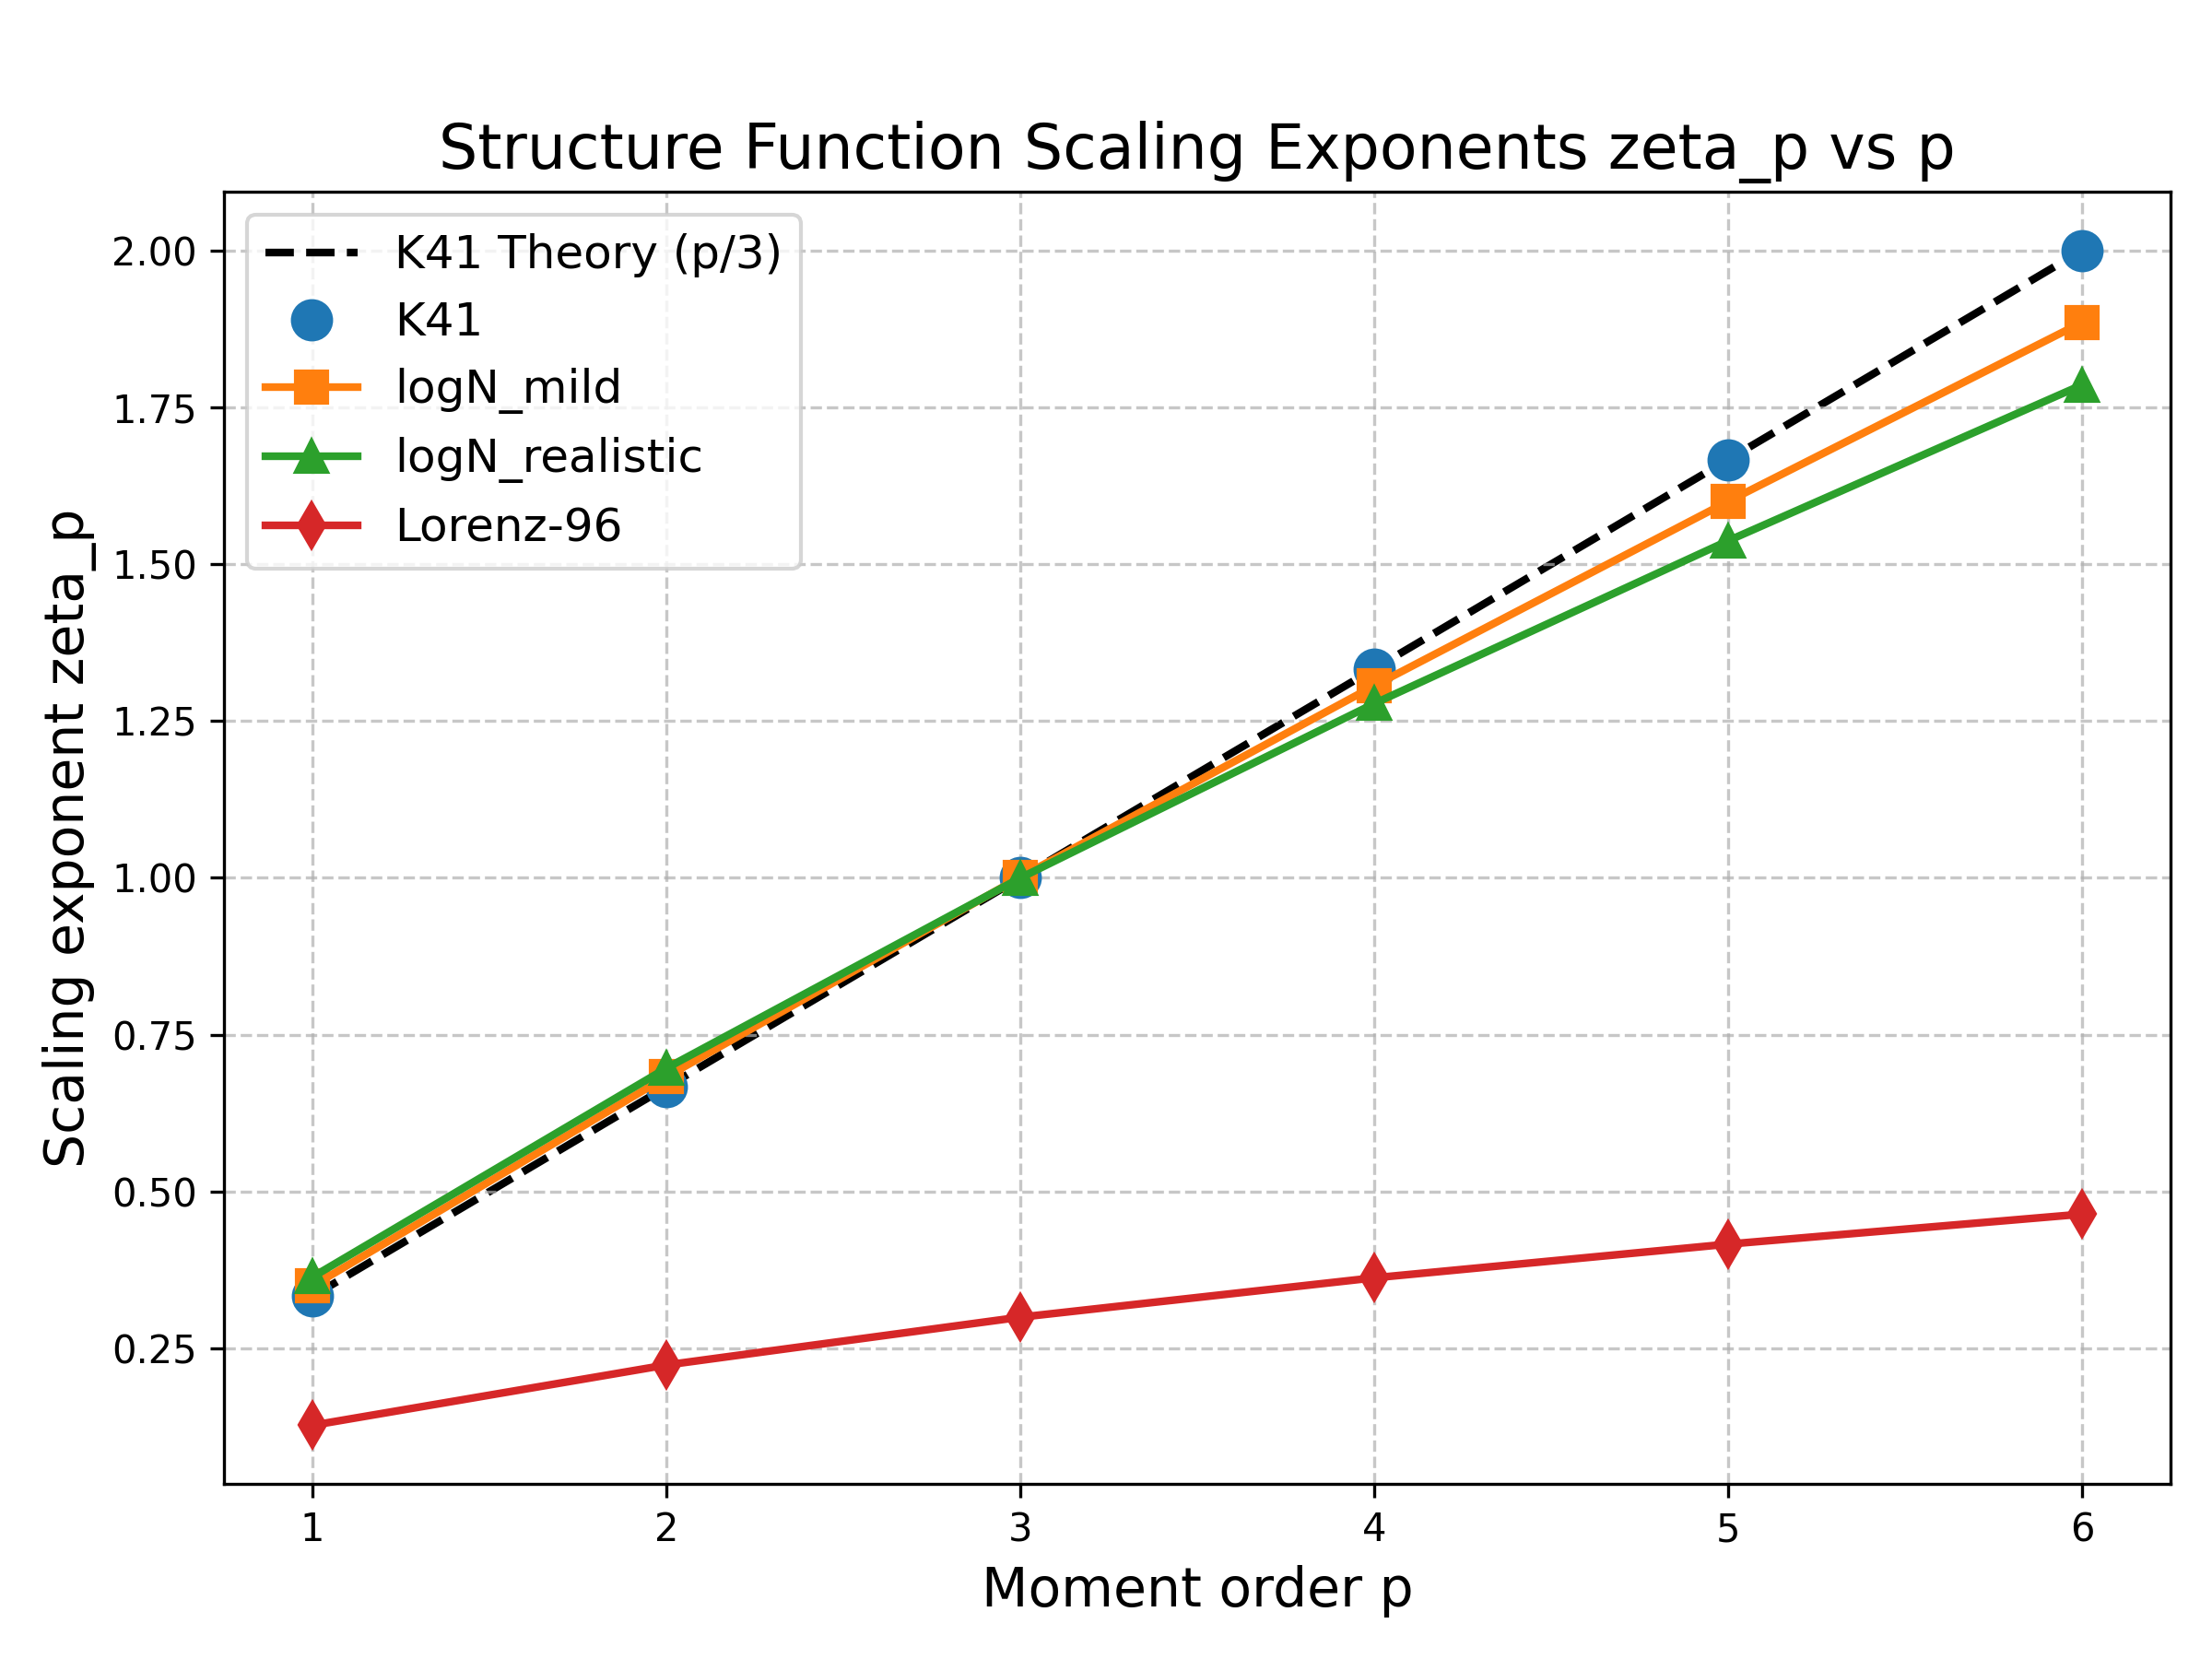
\includegraphics[width=0.5\textwidth]{../input_files/plots/step_2_zeta_p_vs_p_2_1778360956.png}
    \caption{Scaling exponents $\zeta_p$ of the Eulerian velocity structure functions versus the moment order $p$ for several turbulence models. The empirical data for the pure Kolmogorov (K41) cascade align with the theoretical linear scaling $\zeta_p = p/3$. The introduction of intermittency via log-normal models (logN\_mild, logN\_realistic) results in the characteristic nonlinear, concave curvature, with the deviation from linearity increasing with the level of intermittency. In contrast, the deterministic Lorenz-96 model exhibits a significantly flatter scaling profile. These results demonstrate that intermittency systematically increases the second-order exponent $\zeta_2$, and therefore the Eulerian spectral roughness $\xi$, which is used to predict the nature of the Lagrangian transport.}
    \label{fig:zeta_p}
\end{figure}

\subsection{Lagrangian temporal correlations}

A key assumption underlying the theoretical link between Eulerian roughness and fractional diffusion is that the Lagrangian velocity statistics are approximately white-in-time. This ensures that any observed anomalous transport arises from the long-range spatial correlations of the velocity field, rather than from temporal memory effects. To verify this condition, we computed the Lagrangian velocity autocorrelation function, $R_v(\tau)$, for the models used to generate tracer trajectories.

As shown in Figure~\ref{fig:autocorr}, the velocity fields in both the Kraichnan and Lorenz-96 models decorrelate rapidly. For the Kraichnan model, which is constructed to be delta-correlated in time, the autocorrelation function drops to zero within a single time step, as expected. The deterministic Lorenz-96 system also exhibits a very short correlation time ($\tau_c = 0.23$) relative to the total simulation duration ($T=500$). The satisfaction of this white-noise condition is critical, as it allows us to isolate the impact of the spatial structure of the flow on the Lagrangian dynamics.

\begin{figure}[h!]
    \centering
    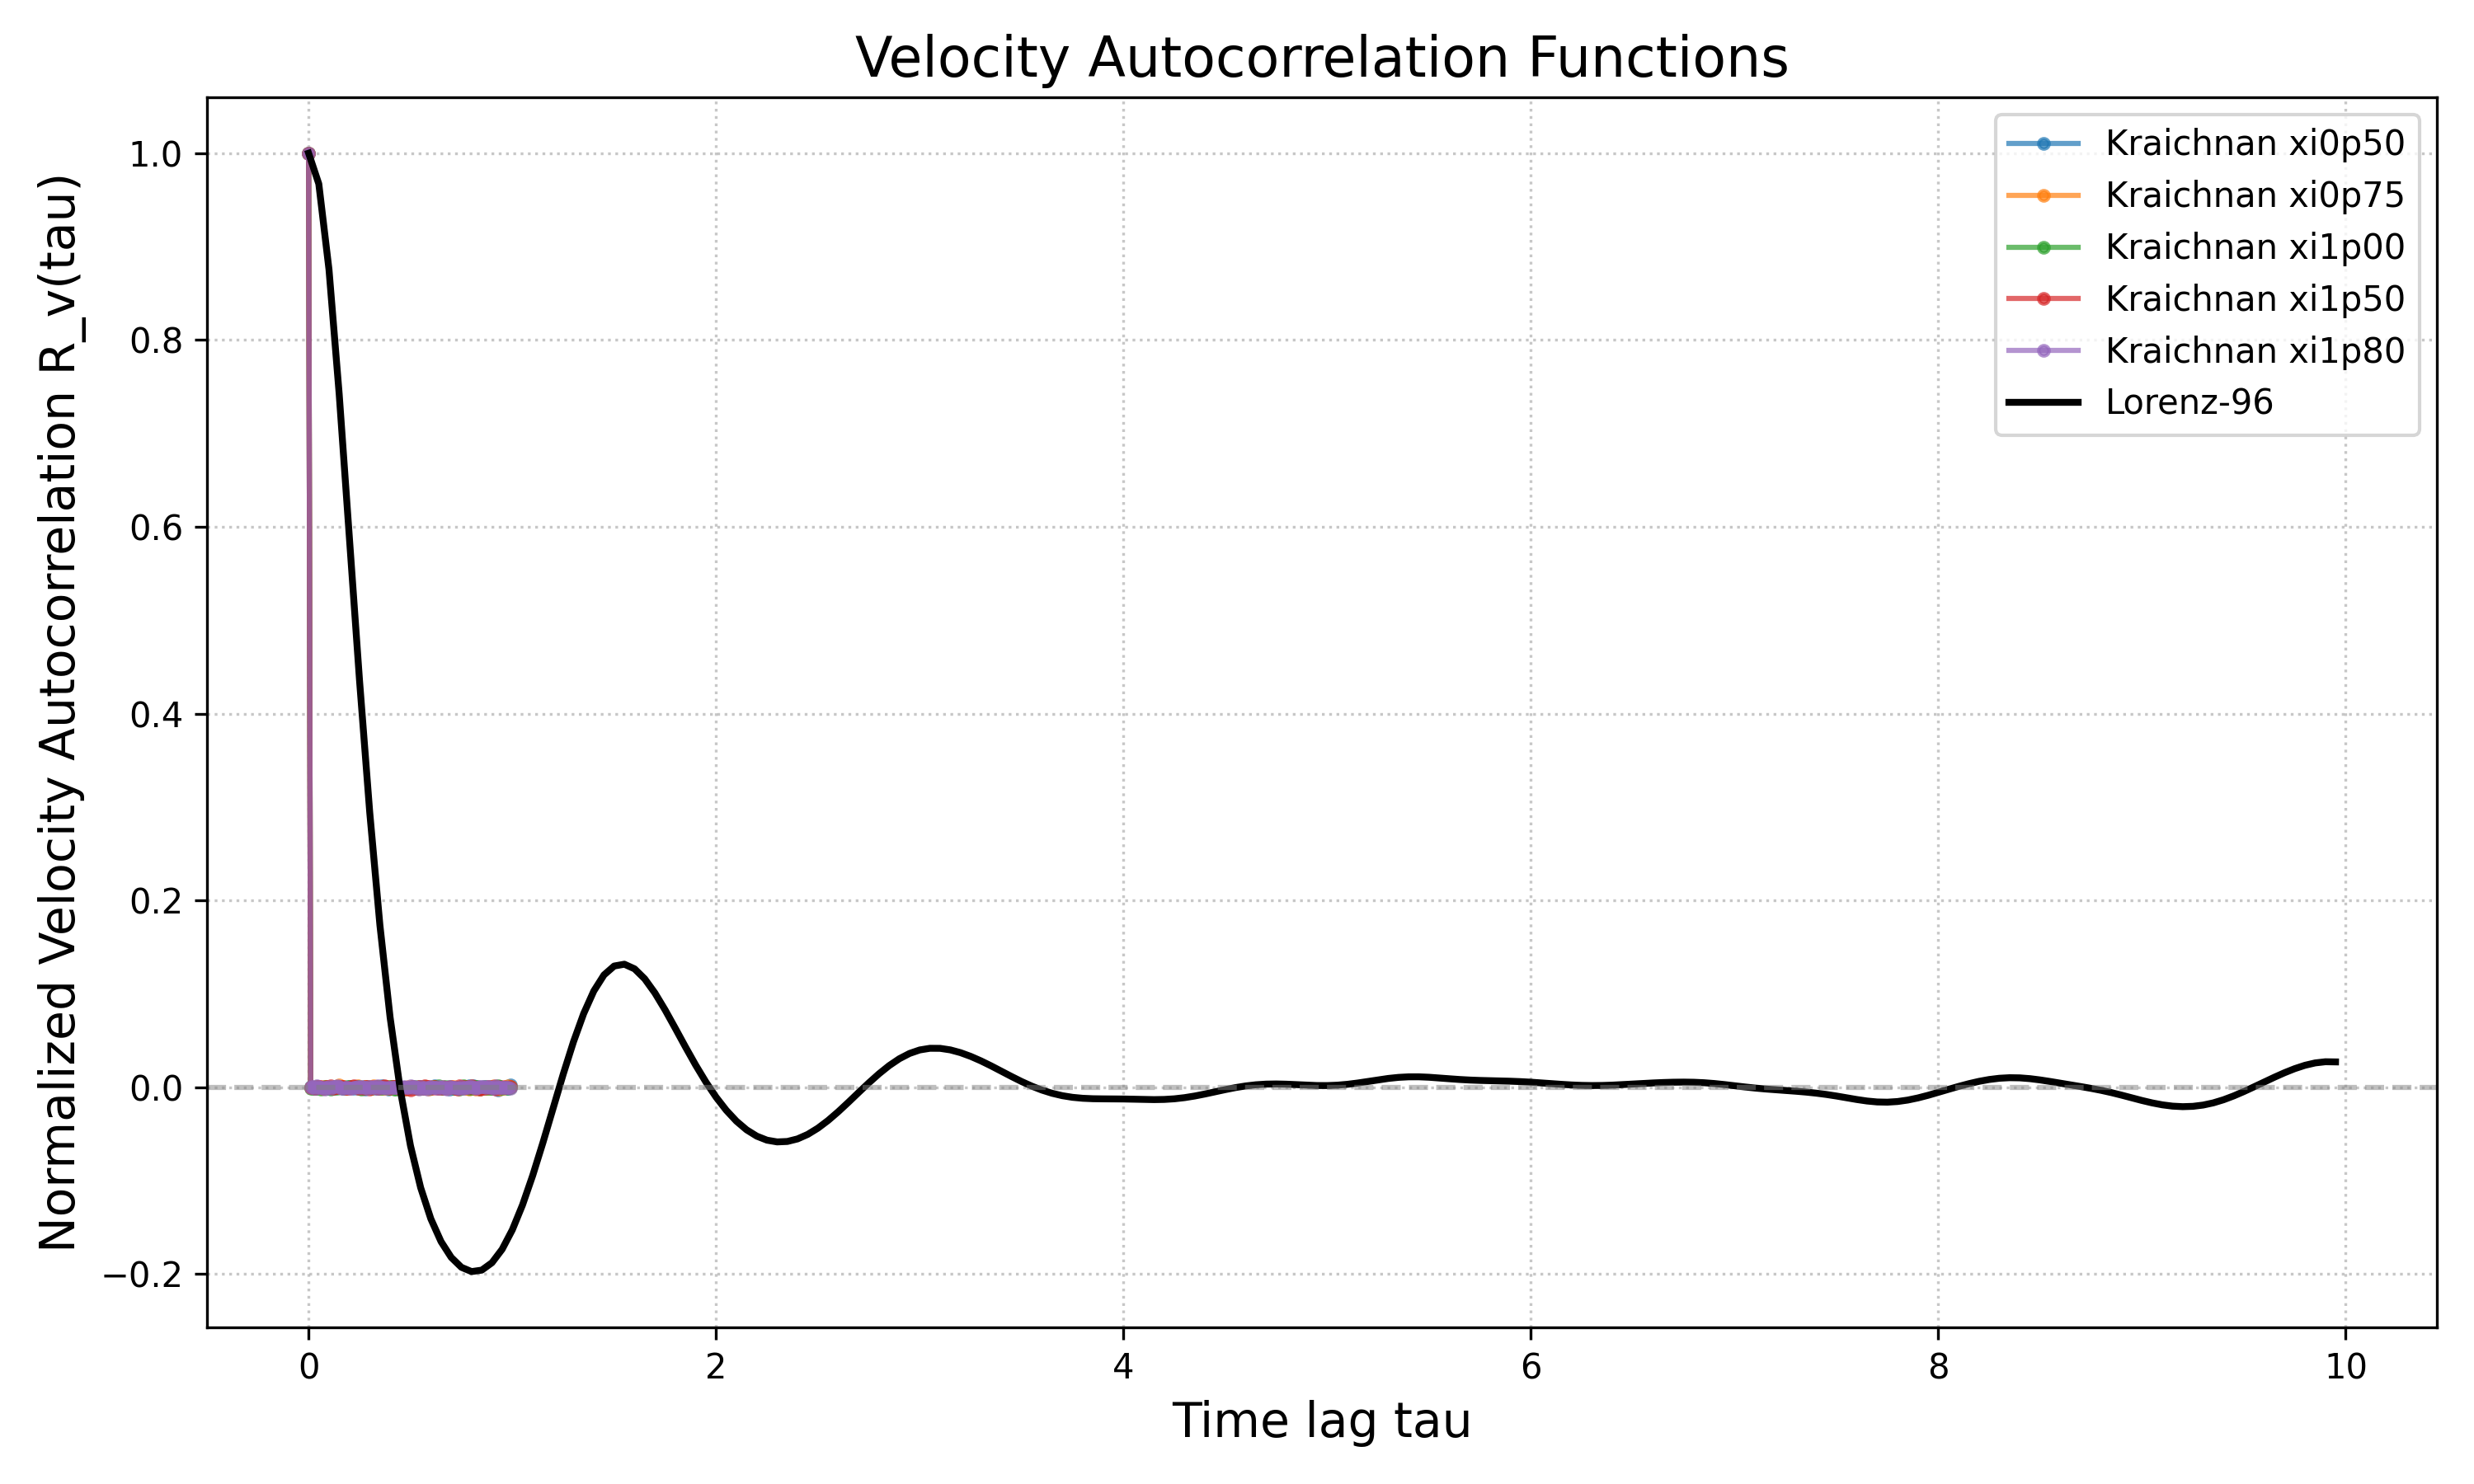
\includegraphics[width=0.5\textwidth]{../input_files/plots/step_3_velocity_autocorr_3_1778361095.png}
    \caption{Lagrangian velocity autocorrelation functions, $R_v(\tau)$, for the Kraichnan model across various spectral roughness exponents ($\xi$) and for the deterministic Lorenz-96 model. The plot demonstrates that the velocity fields in both systems are effectively delta-correlated in time. For the Kraichnan model, the correlation drops instantaneously to zero, reflecting its construction. The Lorenz-96 model also exhibits a rapid decay to zero. This confirmation of the white-in-time approximation is a critical prerequisite, ensuring that observed anomalous diffusion is a consequence of the spatial velocity structure rather than temporal memory effects.}
    \label{fig:autocorr}
\end{figure}

\subsection{Pre-asymptotic constraints on Lagrangian transport in the Kraichnan model}

Having established the Eulerian predictions and verified the necessary temporal conditions, we next examined the Lagrangian transport statistics in the 3D Kraichnan model. This synthetic model serves as an ideal testbed, as the spectral roughness $\xi$ can be precisely controlled. The theory predicts superdiffusive transport, with the Mean Squared Displacement (MSD) scaling as $\langle \Delta x^2(\tau) \rangle \propto \tau^{2H}$ where the Hurst exponent $H = \xi/2$, and a displacement distribution characterized by a Lévy index $\alpha = 2/\xi$.

However, our empirical results show a significant departure from these asymptotic predictions. Figure~\ref{fig:kraichnan_msd} displays the MSD for several values of $\xi$. In all cases, the measured Hurst exponent remains close to $H \approx 0.5$, the value characteristic of normal, classical diffusion. This result stands in stark contrast to the theoretical predictions of strong superdiffusion (e.g., $H=0.75$ for $\xi=1.5$).

\begin{figure}[h!]
    \centering
    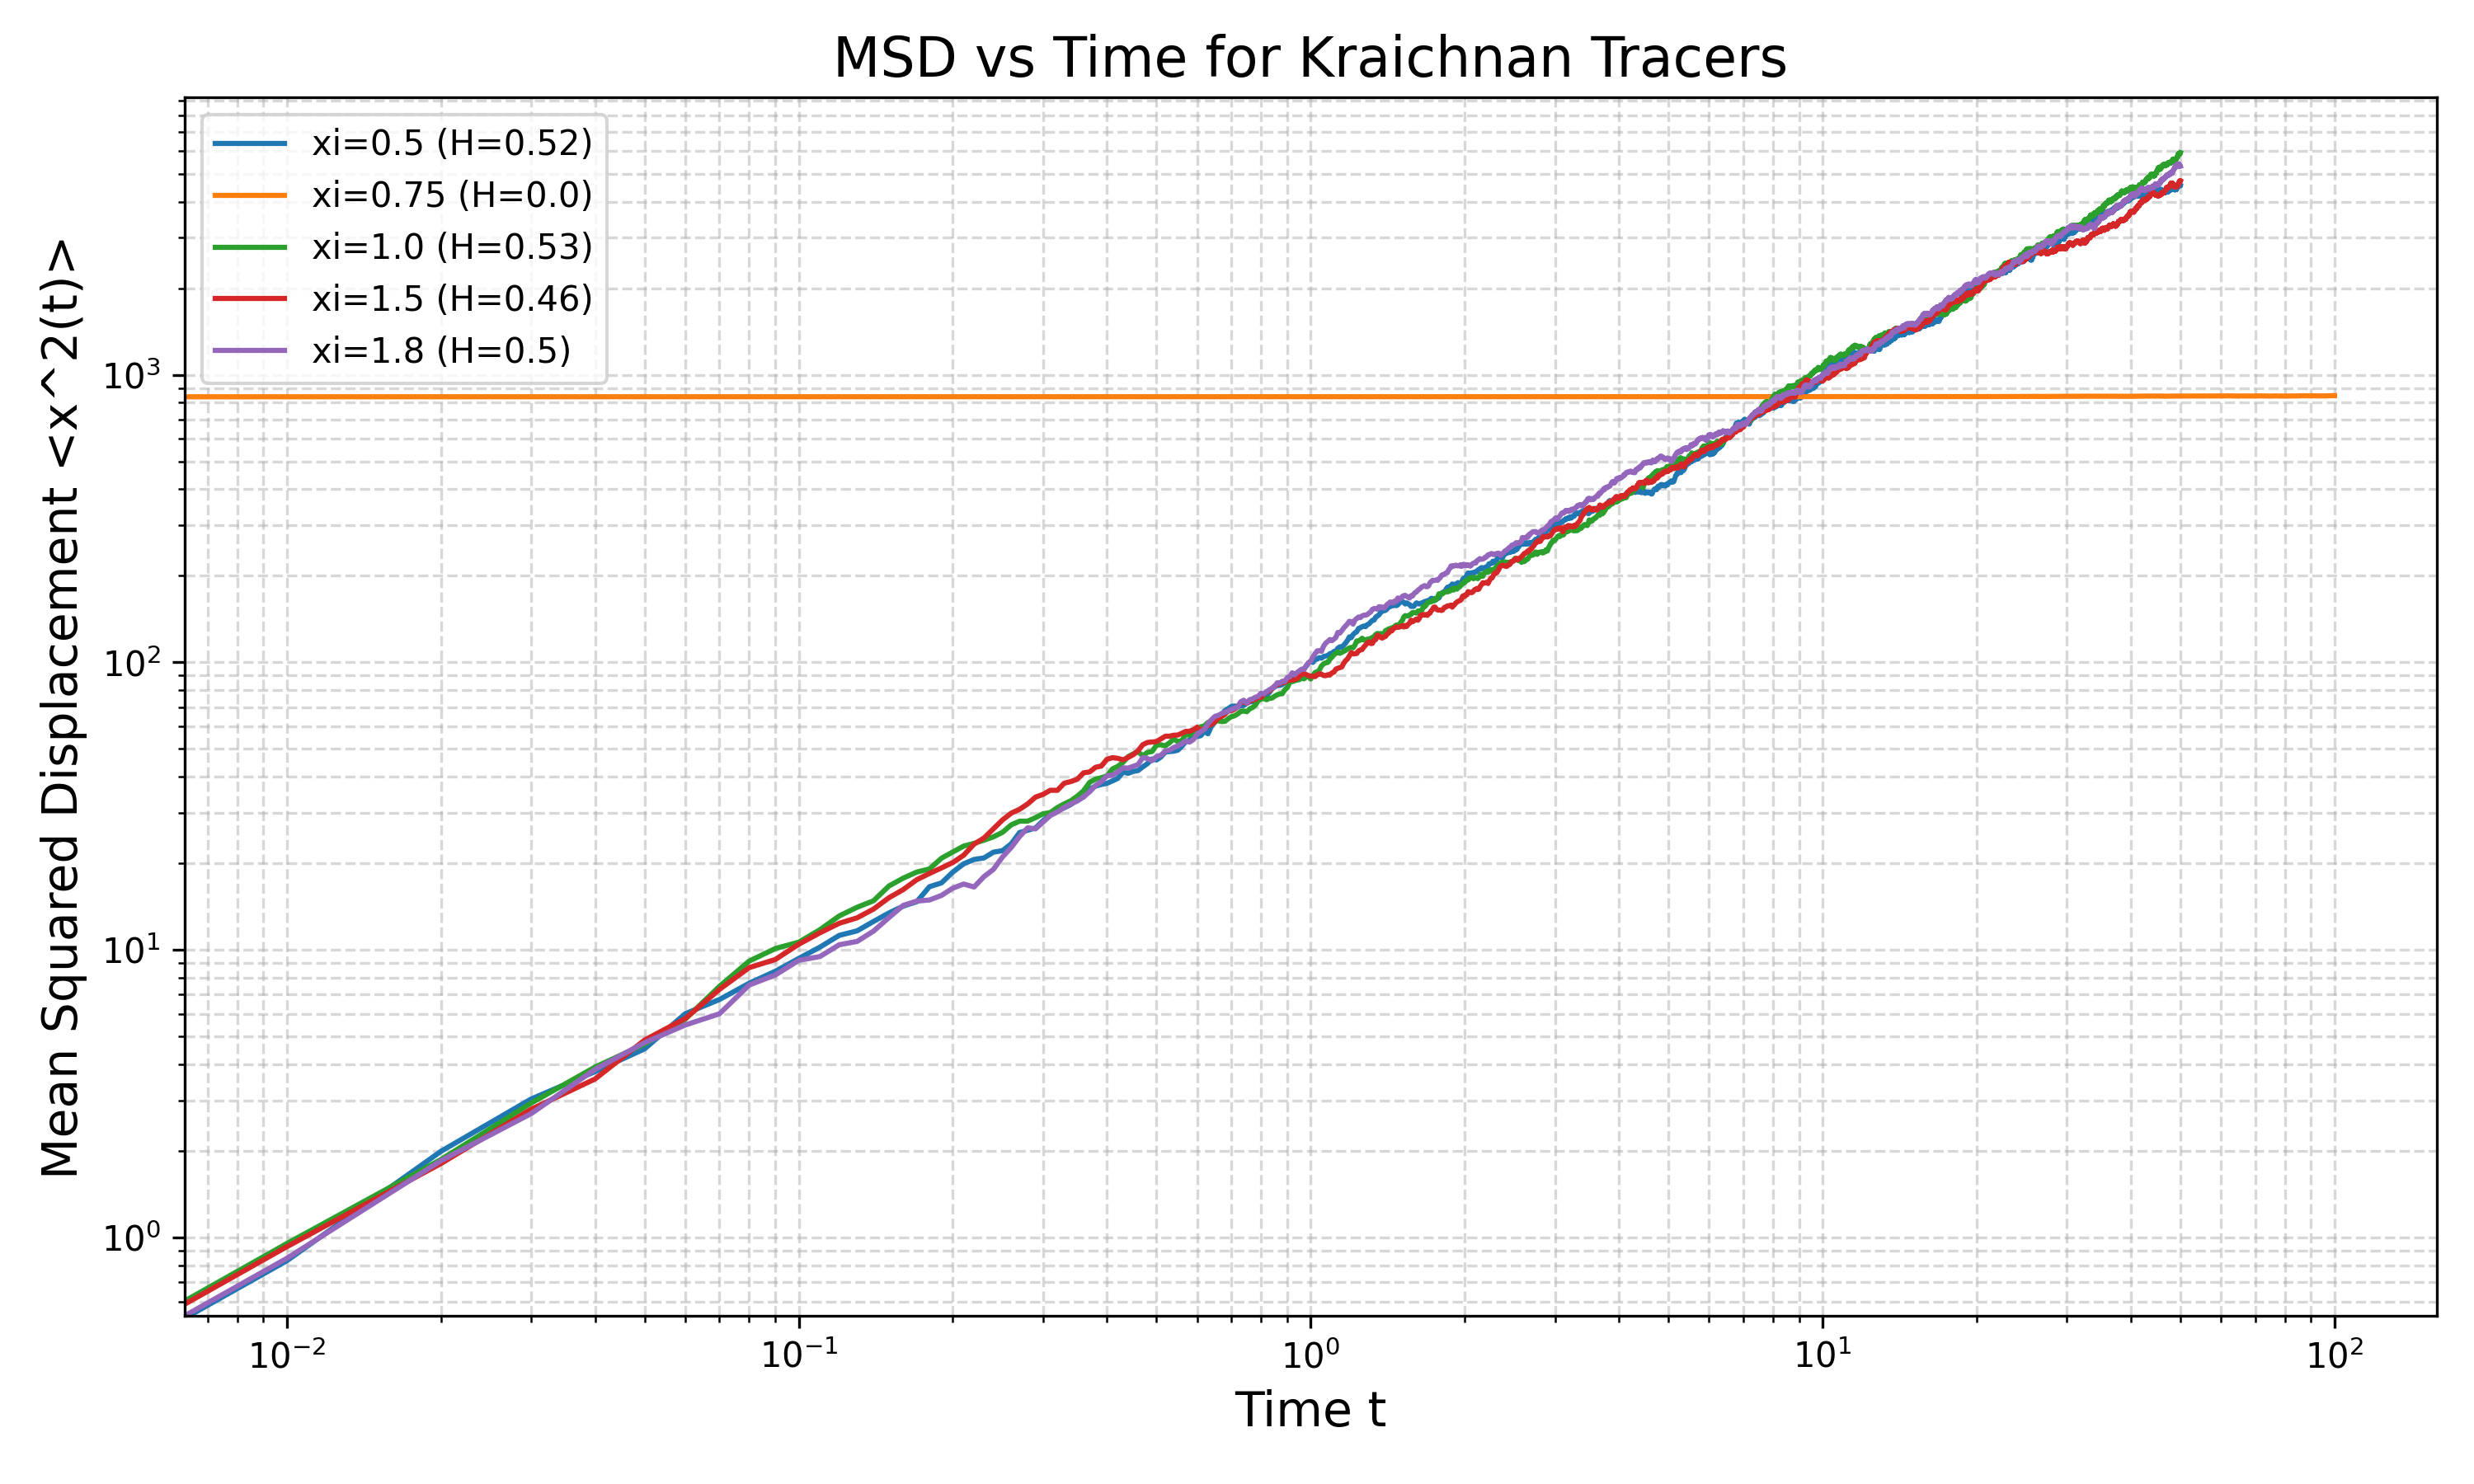
\includegraphics[width=0.5\textwidth]{../input_files/plots/step_4_kraichnan_msd_4_1778361306.png}
    \caption{Log-log plot of the Mean Squared Displacement (MSD) versus time for Lagrangian tracers in the 3D Kraichnan model, shown for several values of the Eulerian spectral roughness exponent $\xi$. The legend displays the empirically measured Hurst exponent, $H$, for each case. Contrary to the theoretical prediction of anomalous diffusion where $H = \xi/2$, the measured scaling exponents consistently remain near $H \approx 0.5$, which is characteristic of normal diffusion. This reveals that the system is trapped in a pre-asymptotic state, where the finite size of the simulation's spectral domain prevents the tracers from experiencing the long-range correlations required to manifest the true anomalous scaling within the observed time frame.}
    \label{fig:kraichnan_msd}
\end{figure}

This near-diffusive behavior is further reflected in the shape of the Probability Density Functions (PDFs) of particle displacements, shown in Figure~\ref{fig:kraichnan_pdf}. The PDFs are dominated by a Gaussian-like central bulk and lack the pronounced heavy tails that are the hallmark of Lévy-stable processes. To quantify this, we directly estimated the Lévy index $\alpha$ from the displacement data. As shown in the Hill plots in Figure~\ref{fig:hill_plots}, the estimators for $\alpha$ are highly unstable and fail to converge to the theoretical prediction of $\alpha = 2/\xi$. Instead, they are strongly biased towards the Gaussian limit of $\alpha=2$.

Taken together, these results indicate that the system is trapped in a pre-asymptotic state. The finite spectral resolution of the simulation ($N_k=128$) and the finite simulation time prevent the tracer particles from sufficiently sampling the long-range spatial correlations of the velocity field. Consequently, the dynamics are dominated by the central part of the displacement distribution, and the theoretically predicted fractional behavior does not manifest.

\begin{figure}[h!]
    \centering
    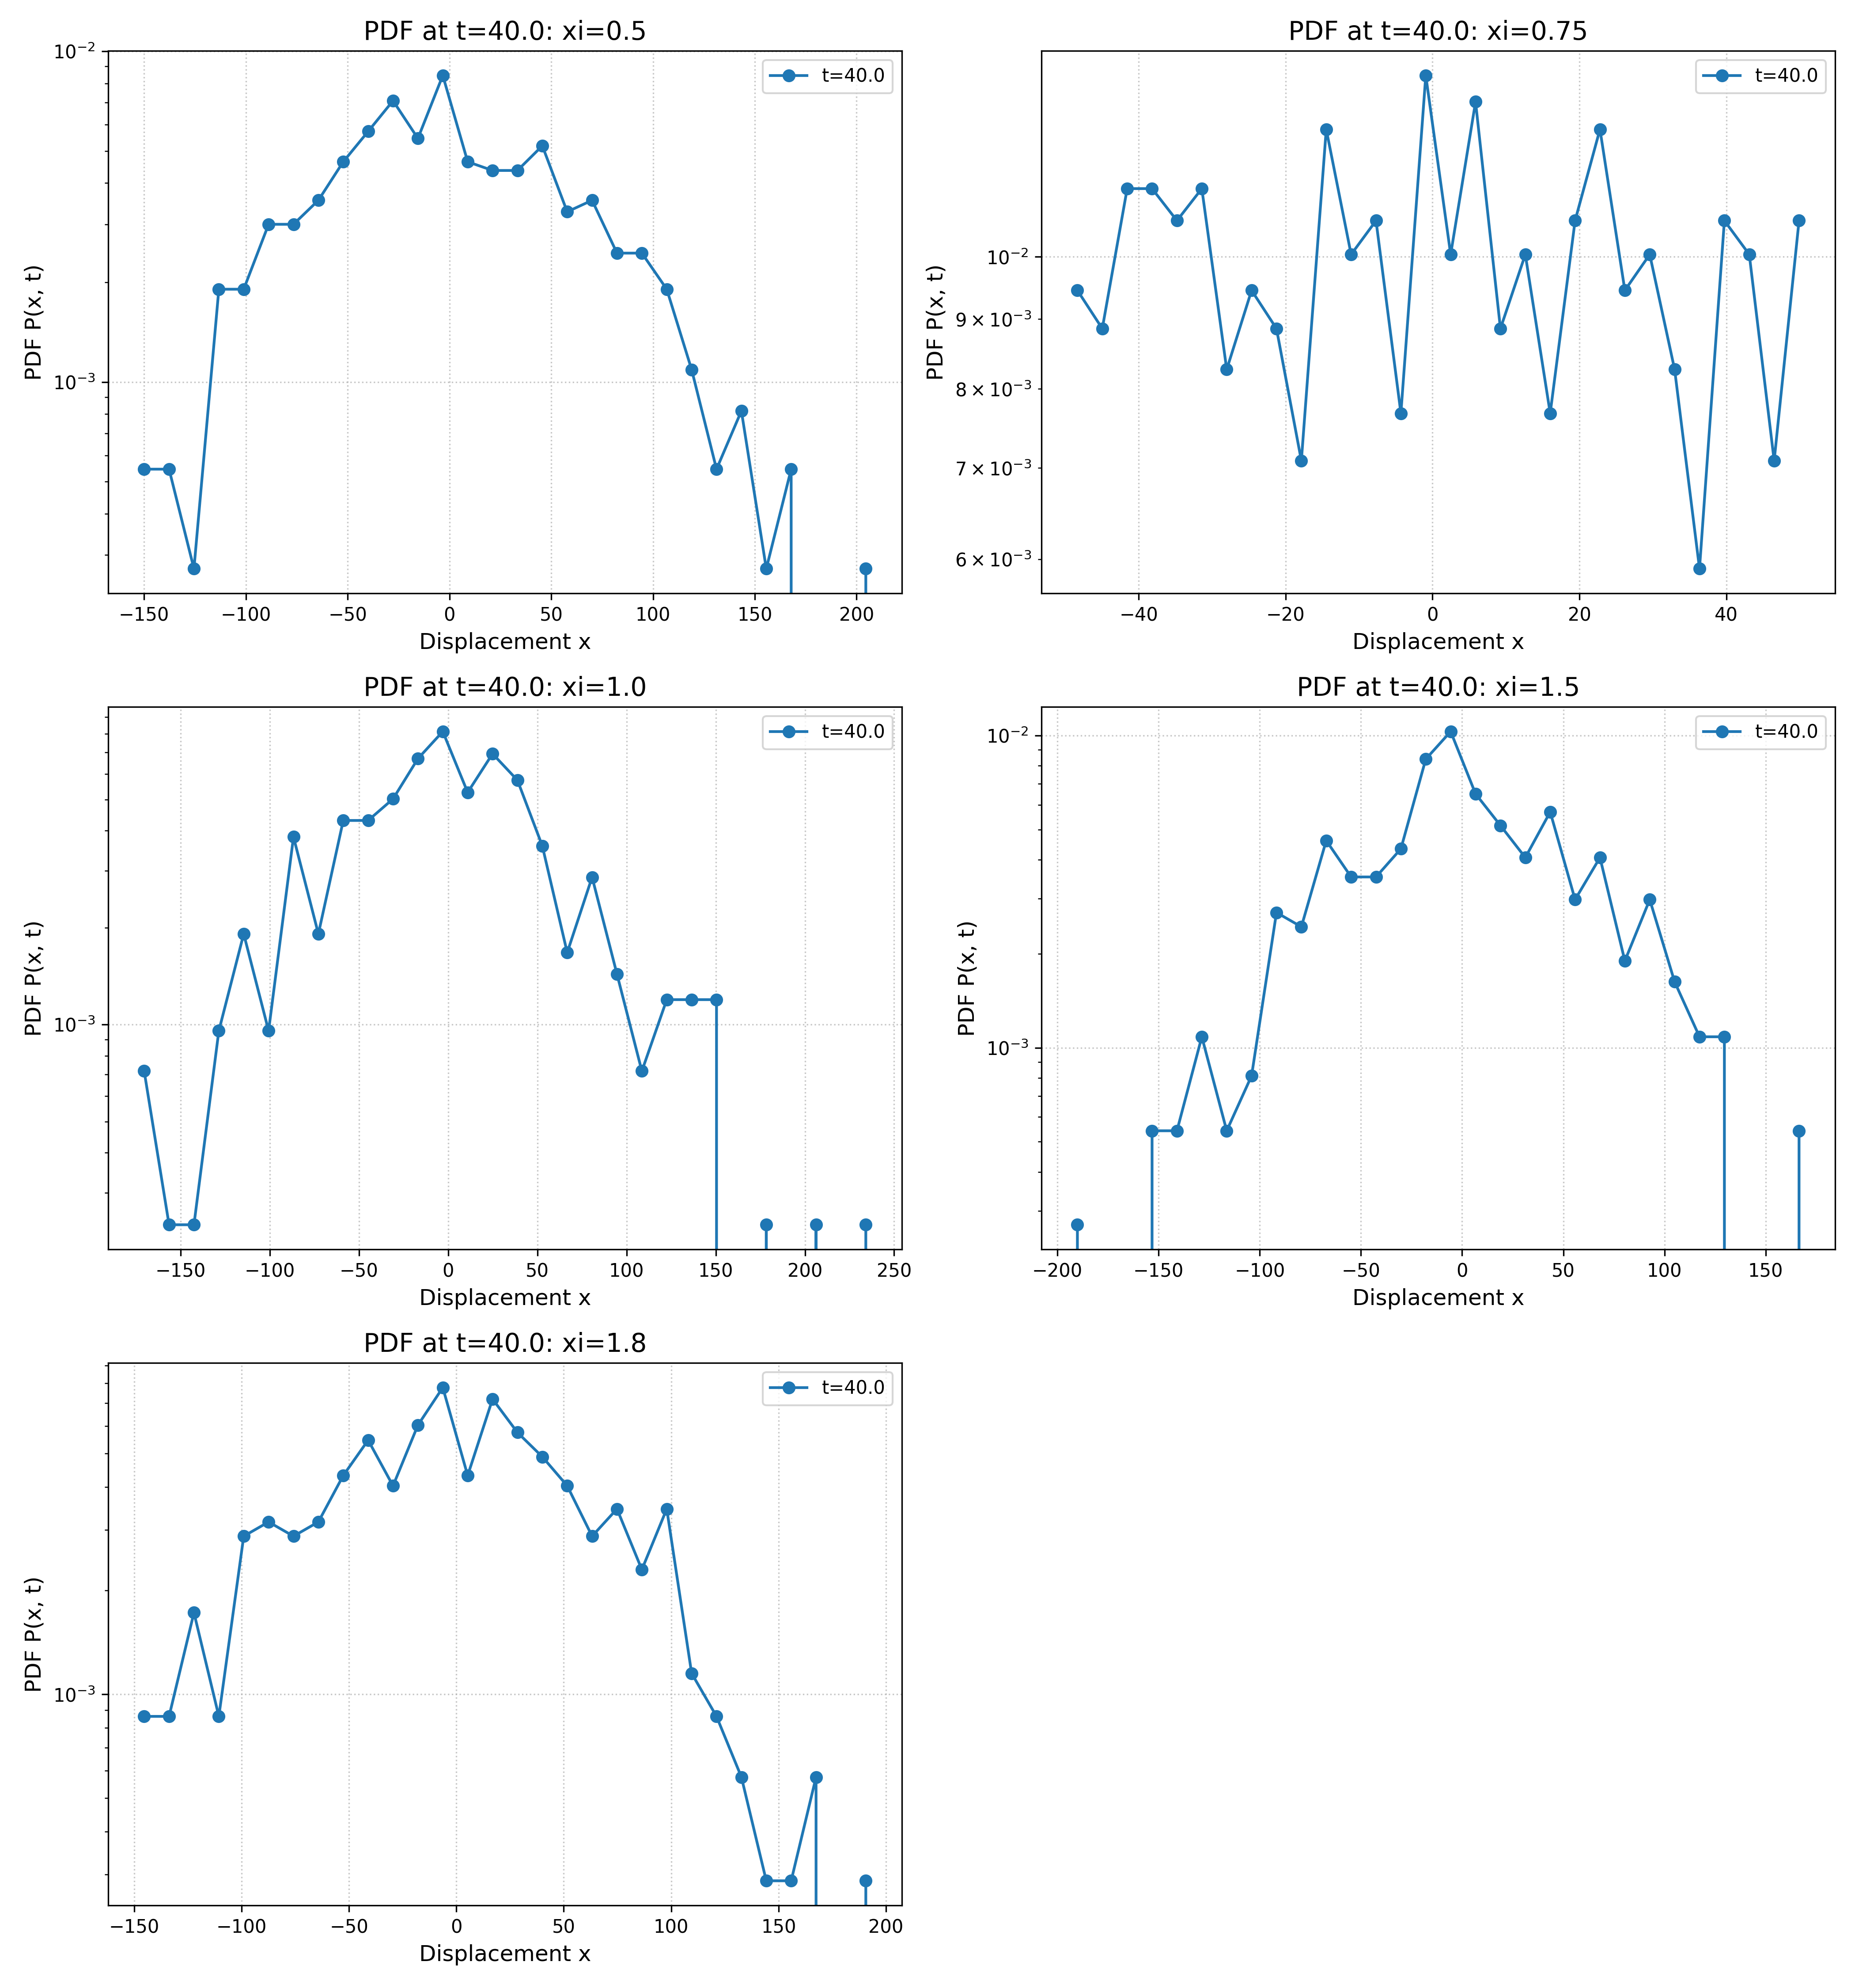
\includegraphics[width=0.5\textwidth]{../input_files/plots/step_4_kraichnan_pdf_4_1778361306.png}
    \caption{Probability Density Functions (PDFs) of Lagrangian tracer displacements at t=40.0 in the Kraichnan model for different Eulerian spectral roughness exponents $\xi$. The distributions show a dominant central bulk, indicating that the system remains in a pre-asymptotic, near-Gaussian regime. This visualizes the impact of finite simulation size, which prevents the emergence of the heavy tails characteristic of the theoretically predicted asymptotic Lévy-stable statistics.}
    \label{fig:kraichnan_pdf}
\end{figure}

\begin{figure}[h!]
    \centering
    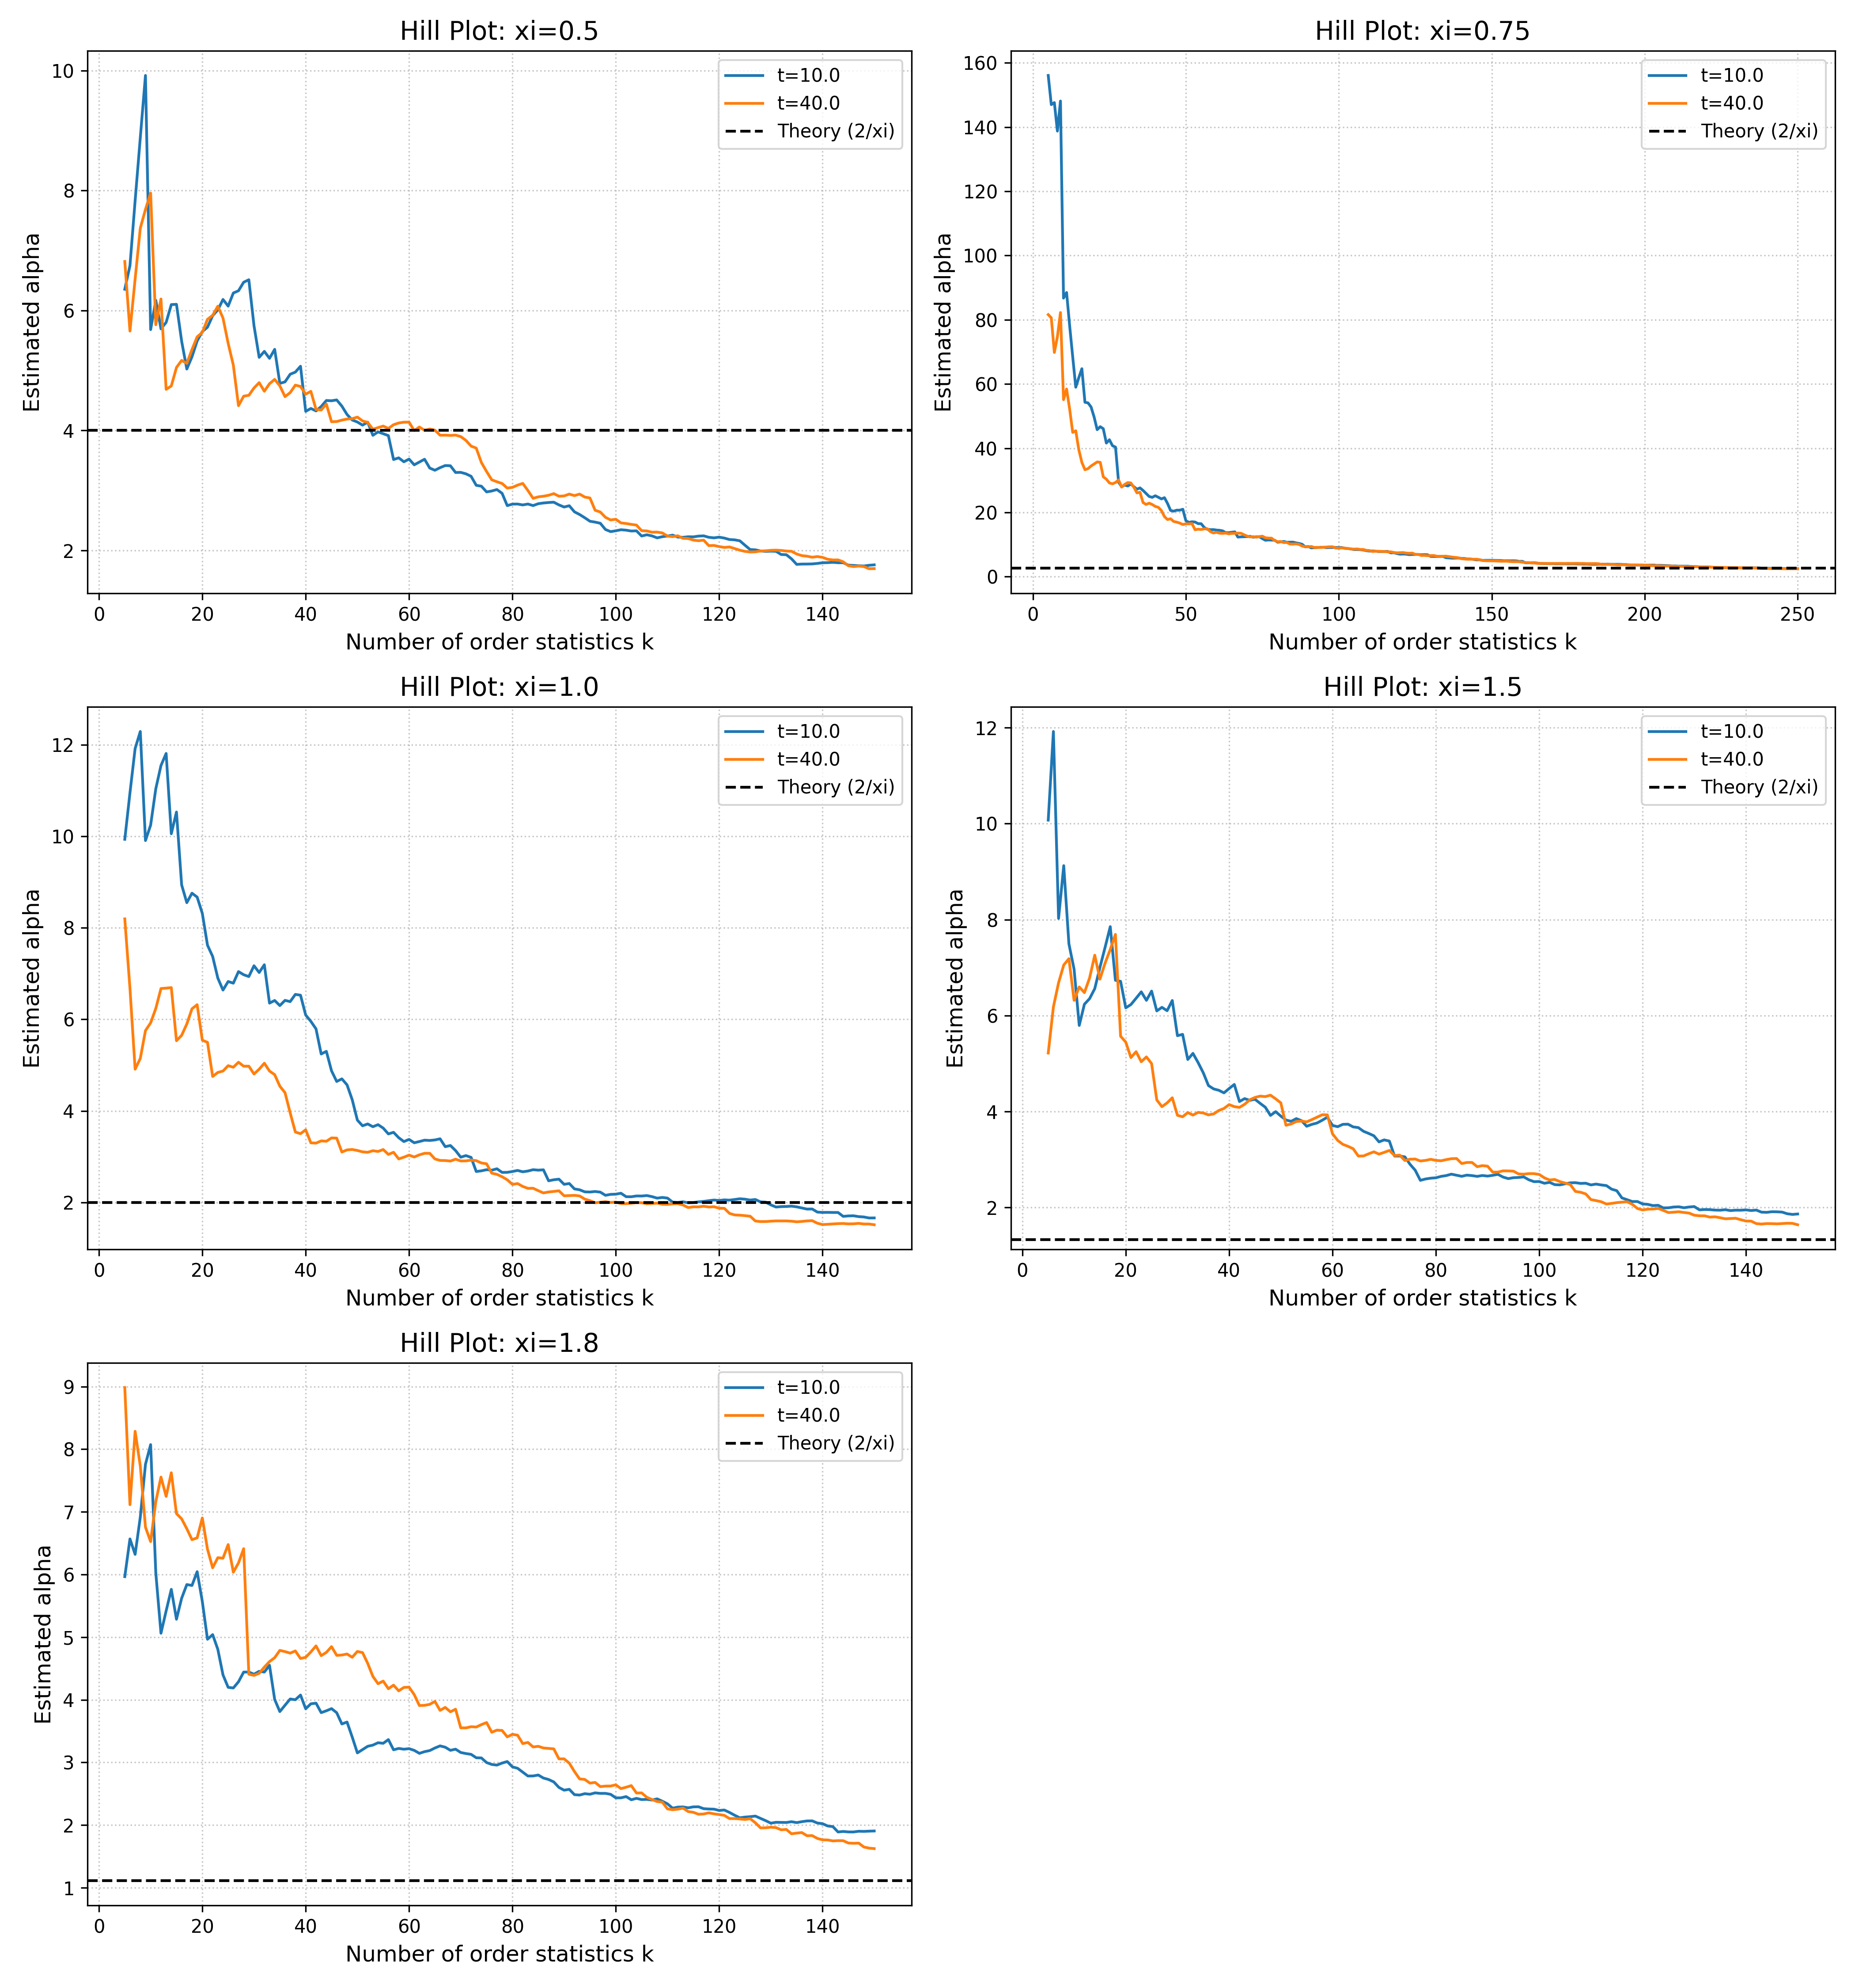
\includegraphics[width=0.5\textwidth]{../input_files/plots/step_4_hill_stability_4_1778361306.png}
    \caption{Hill plots for the estimation of the Lévy index $\alpha$ from tracer displacements in the Kraichnan model across five values of the Eulerian spectral roughness, $\xi$. Each panel shows the estimated $\alpha$ versus the number of order statistics $k$ at two times, compared with the theoretical prediction $\alpha = 2/\xi$ (dashed line). For the anomalous superdiffusive cases ($\xi=1.5$ and $\xi=1.8$), the estimates fail to converge to the theory and are biased towards the Gaussian limit ($\alpha=2$). This demonstrates the pre-asymptotic trapping of the system, where finite-size effects cause the Gaussian bulk of the displacement distribution to dominate the expected fractional tails.}
    \label{fig:hill_plots}
\end{figure}

\subsection{Renormalization group flow analysis}

To directly visualize the system's failure to reach the asymptotic fractional regime, we tracked the Renormalization Group (RG) flow of the effective Lévy exponent, $\alpha(\tau)$, as a function of the time lag $\tau$. This approach allows us to observe whether the system evolves from its short-time behavior towards the predicted fixed point. We extracted $\alpha(\tau)$ by fitting the empirical characteristic function of the displacements at each time lag.

The scaling of the characteristic function, $\phi(k, \tau)$, is shown in Figure~\ref{fig:char_func}. For a Lévy-stable process, the negative logarithm of $\phi(k, \tau)$ should scale as $|k|^{\alpha(\tau)}$. The plot reveals that the slopes of the curves are nearly identical and parallel for all time lags, indicating that the effective exponent $\alpha(\tau)$ remains constant.

\begin{figure}[h!]
    \centering
    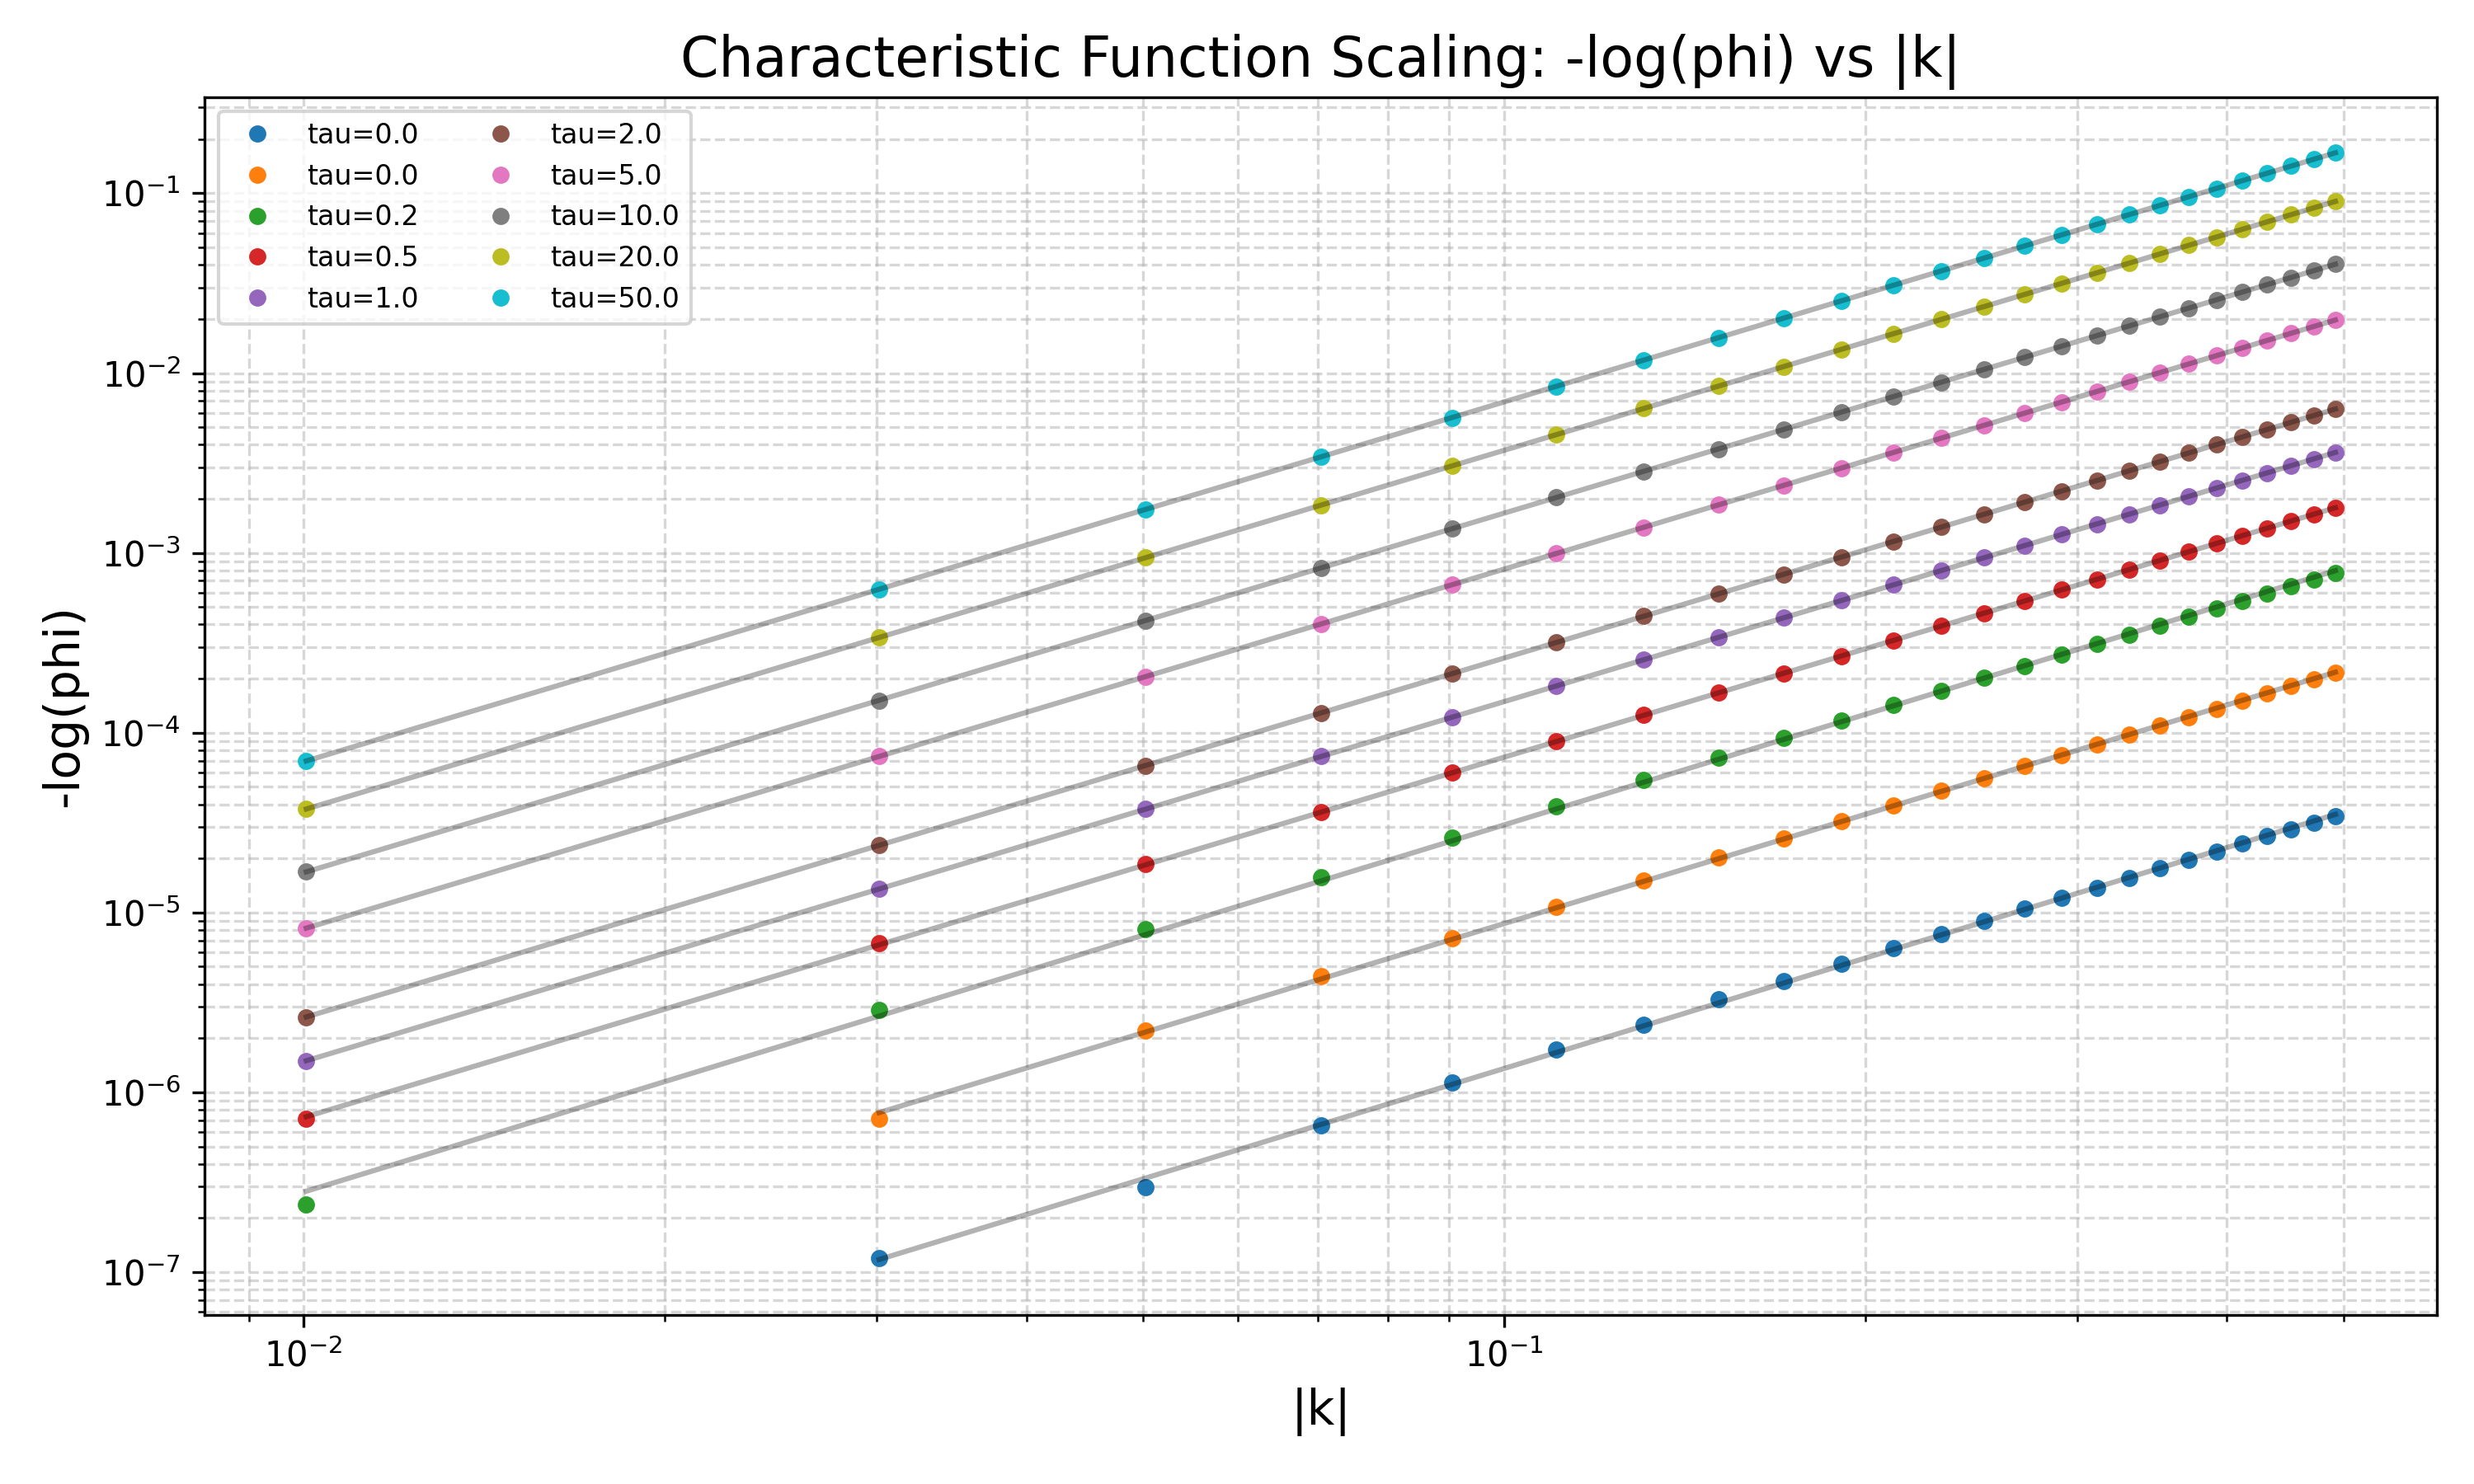
\includegraphics[width=0.5\textwidth]{../input_files/plots/step_5_char_func_scaling_5_1778361494.png}
    \caption{Scaling of the characteristic function $\phi(k, \tau)$ for different time lags $\tau$ in the Kraichnan model, plotted as the negative logarithm of the characteristic function versus wavenumber $|k|$ on a log-log scale. The slope of each line corresponds to the effective Lévy index $\alpha(\tau)$. The consistent, parallel slopes across all time lags ($\tau \in [0.01, 50.0]$) provide direct evidence that the system remains in a pre-asymptotic state with a near-constant exponent $\alpha(\tau) \approx 2.0$. This demonstrates that the Renormalization Group flow does not reach the predicted anomalous diffusive fixed point within the observed simulation time, trapping the dynamics in a near-Gaussian regime.}
    \label{fig:char_func}
\end{figure}

This constant scaling directly translates into the static RG flow plotted in Figure~\ref{fig:rg_flow}. This result provides the most direct evidence of pre-asymptotic trapping. The effective exponent $\alpha(\tau)$ remains robustly pinned near the Gaussian value of $\alpha=2.0$ across the entire range of observed time scales for both the $\xi=1.5$ and $\xi=1.8$ cases. The system shows no tendency to flow towards the theoretically predicted fixed points (dashed lines). This demonstrates that the crossover time required to transition into the anomalous regime is far greater than the total simulation time. The emergence of the fractional dynamics predicted by the Eulerian roughness is thus suppressed by the finite scale separation available in the simulation.

\begin{figure}[h!]
    \centering
    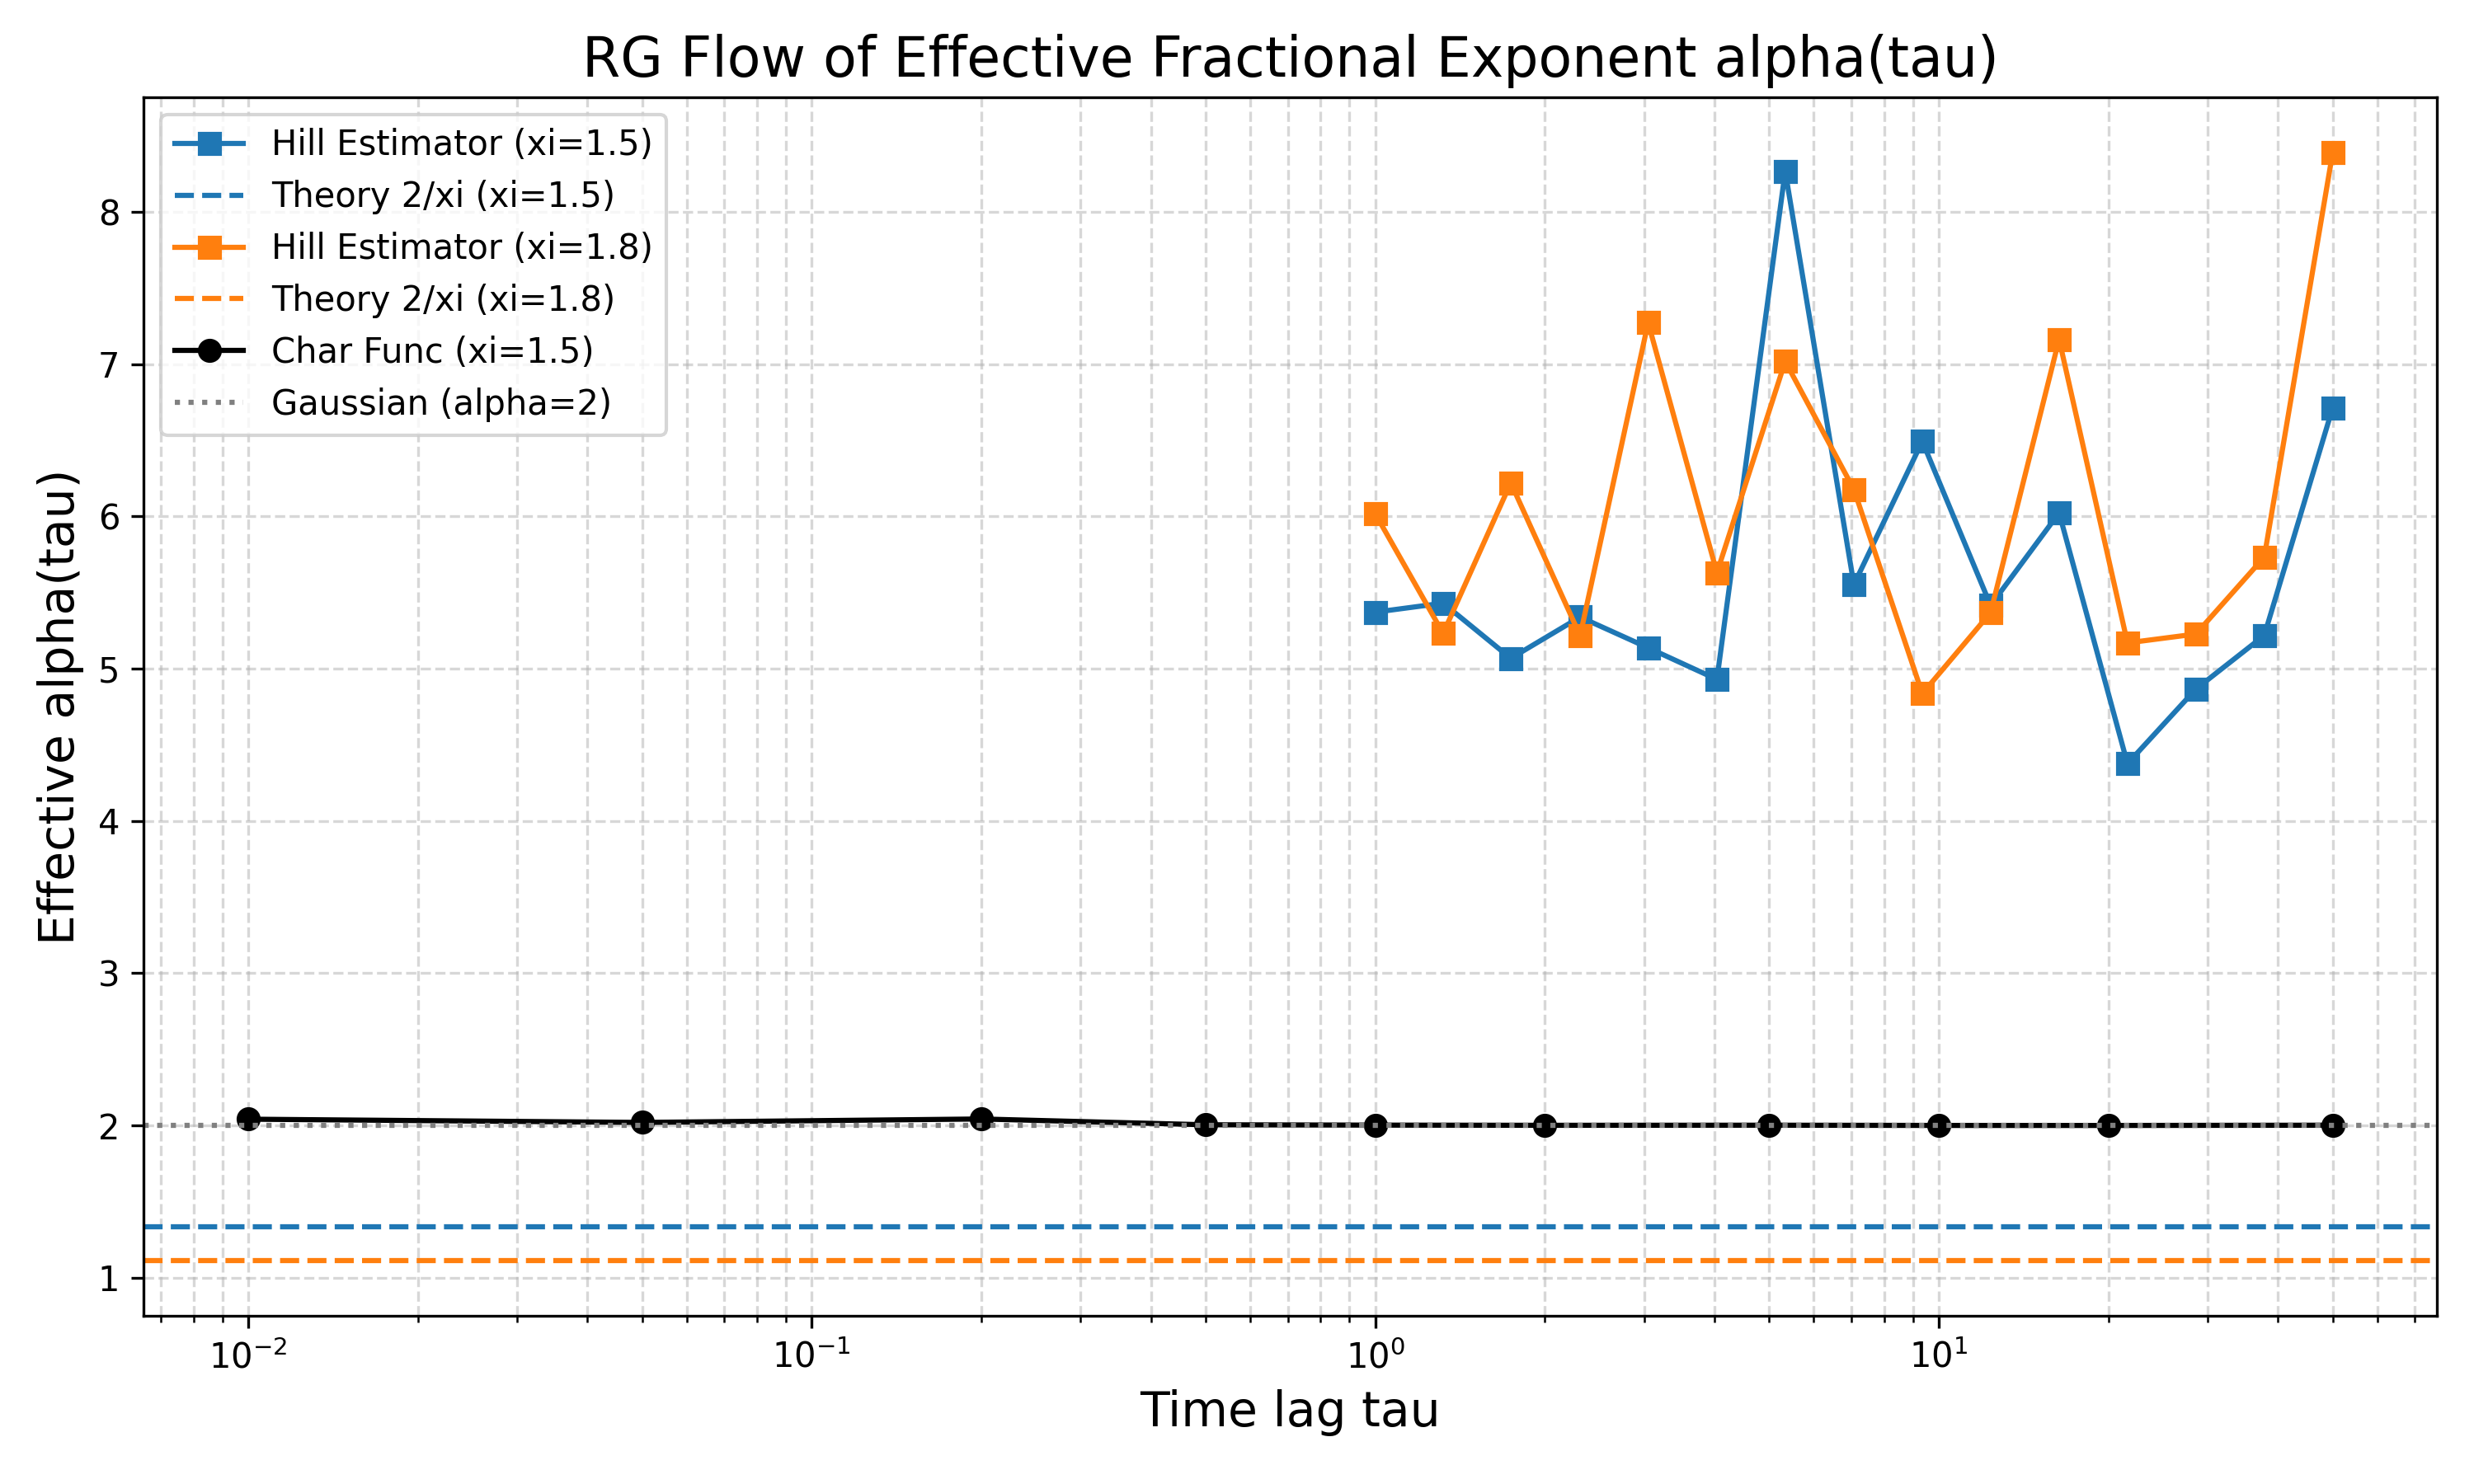
\includegraphics[width=0.5\textwidth]{../input_files/plots/step_5_rg_flow_alpha_5_1778361494.png}
    \caption{Renormalization Group (RG) flow of the effective Lévy index $\alpha(\tau)$ as a function of time lag $\tau$ for Kraichnan model simulations with spectral roughness $\xi=1.5$ and $\xi=1.8$. The empirical exponent, derived from a sliding-window analysis of the characteristic functions (black circles), remains pinned at the Gaussian value $\alpha \approx 2.0$ across the entire range of time lags. This demonstrates a failure to flow towards the theoretically predicted asymptotic fixed points $\alpha = 2/\xi$ (dashed lines), indicating that the simulation remains in a pre-asymptotic state where the crossover time to the fractional Lévy regime is much larger than the observation time.}
    \label{fig:rg_flow}
\end{figure}

\subsection{The role of dimensionality: topological trapping in 1D turbulence}

Finally, we investigated the validity of the $\alpha = 2/\xi$ mapping in a different physical context by analyzing tracer data from a one-dimensional synthetic turbulent flow. While the RG framework does not explicitly depend on dimensionality, the physical realization of transport can be strongly affected by topological constraints.

The results, shown in Figure~\ref{fig:1d_trapping}, reveal a stark breakdown of the theoretical mapping in 1D. For both the pure Kolmogorov and intermittent multifractal cases, the transport is strongly subdiffusive, with measured Hurst exponents of $H \approx 0.49$ and $H \approx 0.14$, respectively. The corresponding Lévy indices are $\alpha \approx 0.385$ and $\alpha \approx 0.439$. These values are drastically different from the superdiffusive prediction of $\alpha \approx 1.2$ derived from the Eulerian roughness.

This discrepancy arises from topological trapping. In a one-dimensional flow, tracer particles lack the freedom to move around regions of low velocity or stagnation points. They become trapped for extended periods, which introduces strong negative correlations in their displacements and suppresses the overall variance. This trapping mechanism dominates the transport dynamics, inducing a non-universal, subdiffusive behavior that is not captured by the theoretical framework relating transport to the field's spectral roughness. This finding highlights that the validity of the $\alpha = 2/\xi$ relation is contingent not only on sufficient scale separation but also on a spatial dimensionality that allows particles to freely sample the velocity field's fluctuations.

\begin{figure}[h!]
    \centering
    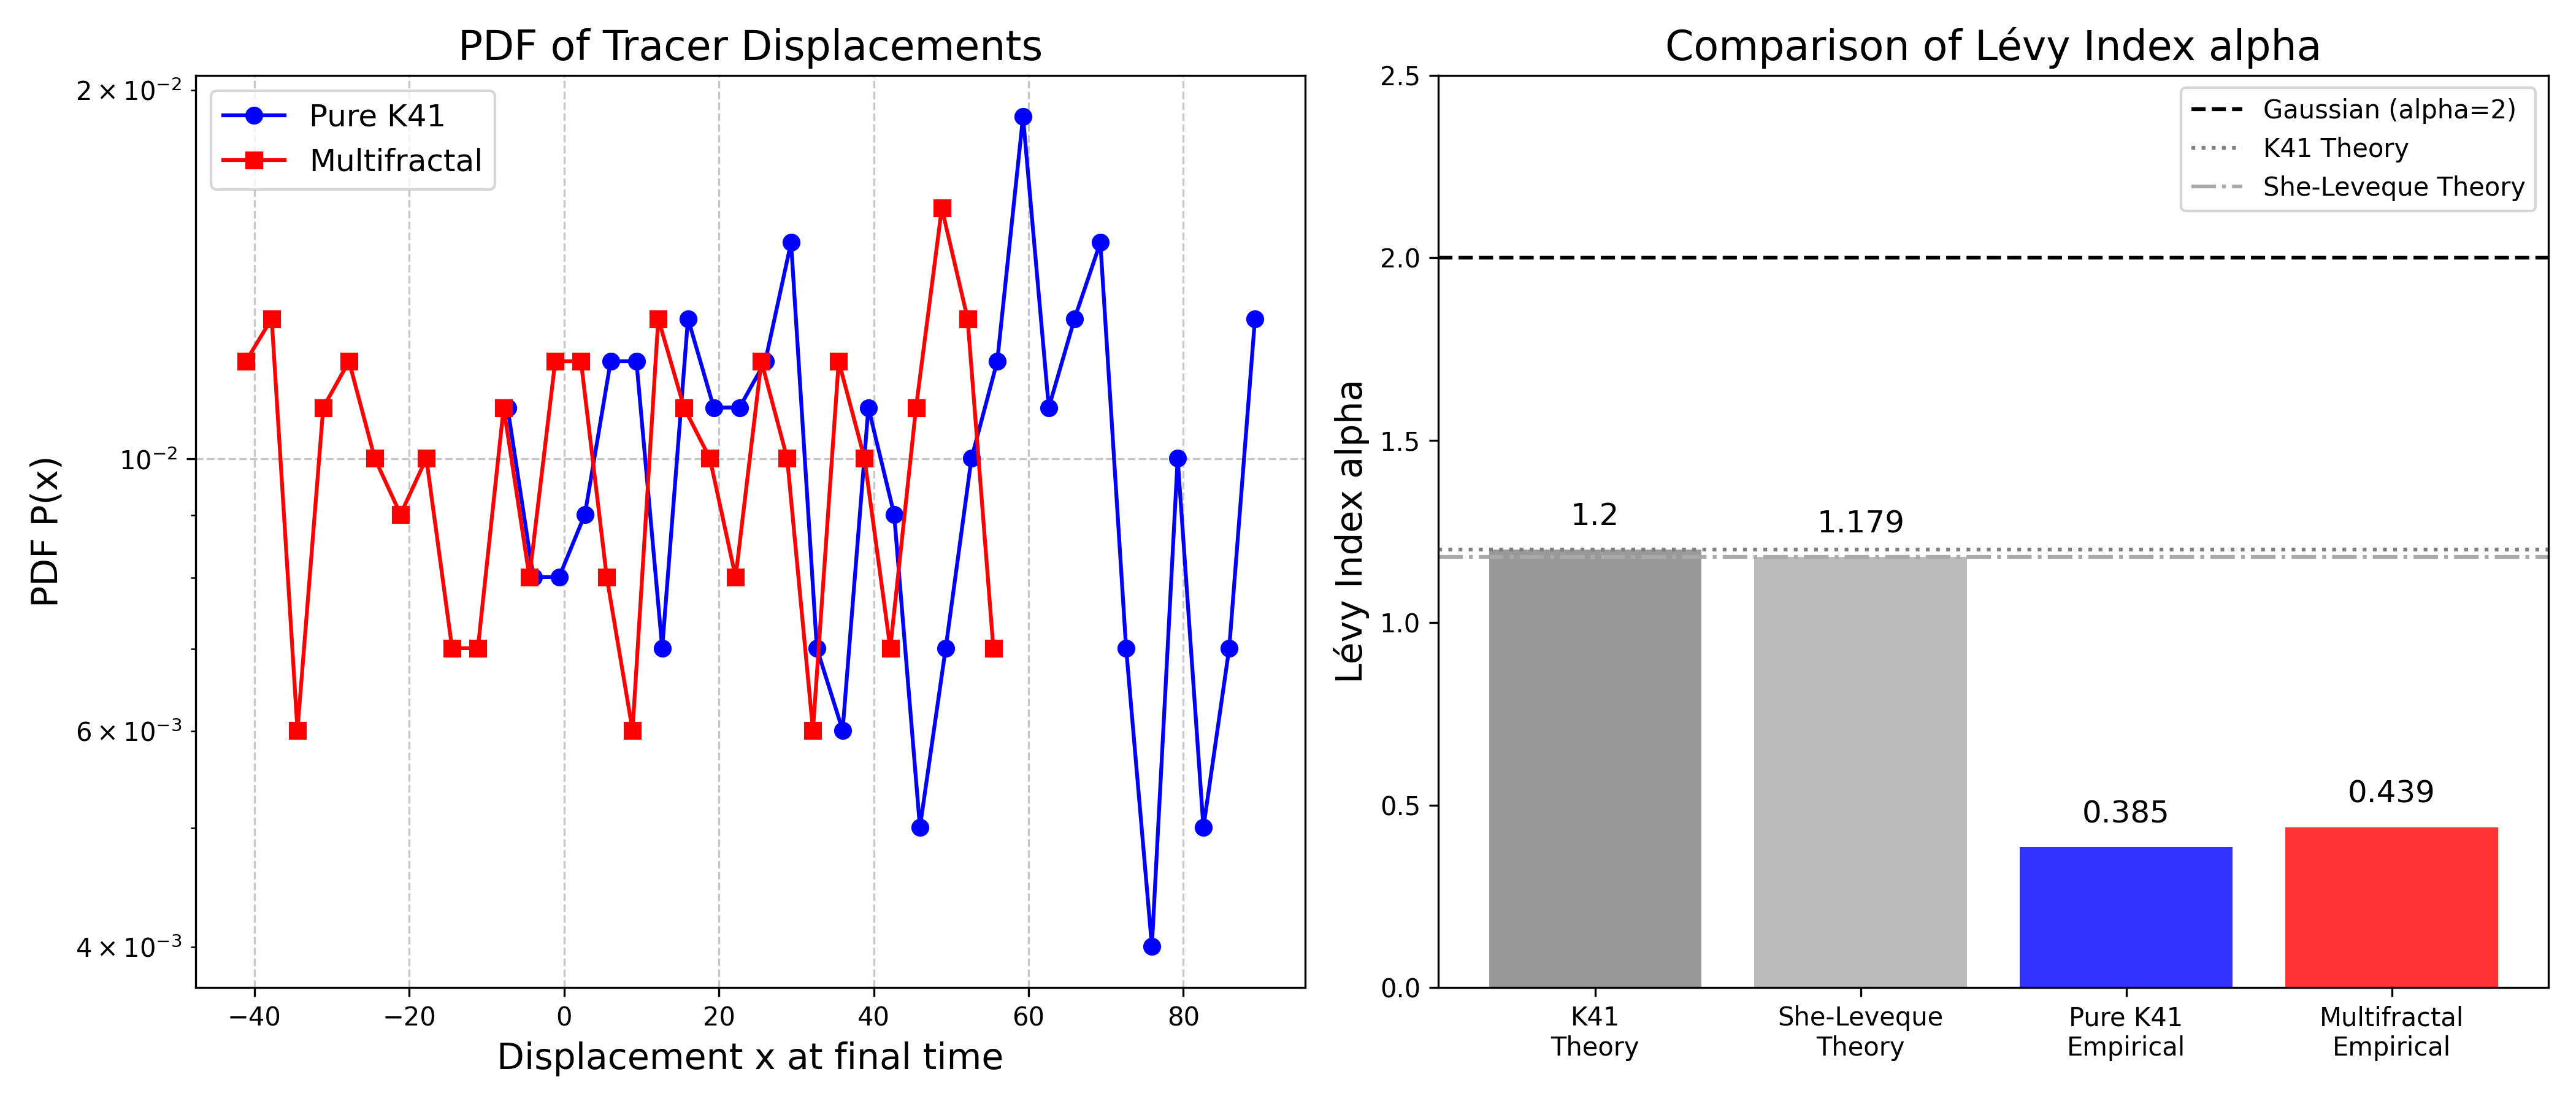
\includegraphics[width=0.5\textwidth]{../input_files/plots/step_6_kolmogorov_intermittency_6_1778360342.png}
    \caption{Analysis of 1D synthetic Kolmogorov tracer data for pure K41 (blue) and multifractal (red) turbulence, showing final displacement Probability Density Functions (left) and a comparison of the Lévy index $\alpha$ (right). The empirical results ($\alpha \approx 0.385$ for pure K41 and $\alpha \approx 0.439$ for multifractal) indicate severe subdiffusion, deviating significantly from the theoretical predictions for Lévy flights derived from the 3D Renormalization Group mapping ($\alpha \approx 1.2$). This discrepancy demonstrates that the theoretical mapping breaks down in 1D due to topological trapping effects that suppress particle transport.}
    \label{fig:1d_trapping}
\end{figure}

\section{Conclusions}
\label{sec:conclusions}
This paper investigated the conditions under which the theoretical asymptotic relationship between Eulerian spectral roughness $\xi$ and the Lagrangian fractional diffusion exponent $\alpha$, given by $\alpha = 2/\xi$, is physically observable in turbulent systems. To address this, we analyzed a hierarchy of numerical models, including multifractal energy cascades, the synthetic Kraichnan model, and the deterministic Lorenz-96 system. Our methodology combined standard Eulerian structure function analysis to determine the predicted roughness $\xi$ with a detailed Lagrangian analysis that tracked the Renormalization Group (RG) flow of an effective, time-dependent exponent $\alpha(\tau)$.

Our Eulerian analysis confirmed that the spectral roughness of the velocity fields behaved as expected, with intermittency systematically increasing the value of $\xi$. This provided a clear theoretical prediction for the corresponding Lagrangian transport. However, the analysis of tracer trajectories in the three-dimensional Kraichnan model revealed a significant departure from this prediction. Despite the theoretical expectation of strong superdiffusion, the transport remained robustly near-diffusive, with the Mean Squared Displacement scaling characteristic of Brownian motion ($H \approx 0.5$) and the displacement distributions lacking the heavy tails of a Lévy process. The RG flow analysis provided a direct visualization of this discrepancy, showing that the effective exponent $\alpha(\tau)$ remained pinned near the Gaussian value of $\alpha=2$ for all accessible time scales, failing to flow towards its predicted anomalous fixed point. This demonstrates that the system was trapped in a pre-asymptotic state, where the finite spectral resolution and simulation duration prevented the emergence of the true fractional dynamics.

Furthermore, our investigation into one-dimensional turbulent flows revealed a fundamental breakdown of the theoretical mapping. In this context, the transport was dominated by a strong, non-universal subdiffusion. This behavior is a direct consequence of topological trapping, a physical mechanism wherein particles are confined for long durations, which is not accounted for in the theoretical framework. This finding underscores that the validity of the theory is contingent on the spatial dimensionality of the system.

From these results, we have learned that while the fractional operator defined by the Eulerian roughness $\xi$ provides a valid, universal description of the asymptotic fixed point of turbulent transport, its physical manifestation is not guaranteed. The emergence of this fractional regime is critically gated by system-specific, pre-asymptotic constraints. First, a sufficient separation of scales and a long enough evolution time are required for the system to cross over from its initial near-Gaussian behavior to the anomalous state. Second, the spatial dimensionality must be sufficient to allow particles to freely sample the velocity field's fluctuations, as topological constraints in lower dimensions can introduce dominant, non-universal transport mechanisms that invalidate the theoretical link. In conclusion, the practical observability of the asymptotic fractional dynamics predicted by the Eulerian field statistics depends critically on whether the physical system can overcome these pre-asymptotic and topological barriers.


\bibliography{bibliography}{}
\bibliographystyle{unsrt}

\end{document}
